%\documentclass[preprint]{sigplanconf}
\documentclass{sigplanconf}

% ICFP 2016:
% By Wednesday, March 16 2016, 15:00 (UTC), submit a full paper of at
% most 12 pages (6 pages for an Experience Report), in standard
% SIGPLAN conference format, including figures but excluding
% bibliography. 

% The following \documentclass options may be useful:

% preprint      Remove this option only once the paper is in final form.
% 10pt          To set in 10-point type instead of 9-point.
% 11pt          To set in 11-point type instead of 9-point.
% authoryear    To obtain author/year citation style instead of numeric.

\usepackage{amsmath,amssymb,amsthm}
\usepackage{stmaryrd}
\usepackage{listings,color}
\usepackage{alltt}
\usepackage{flushend}
\usepackage[utf8]{inputenc} % for proper diacritics: Universität, Hüttel, Luís
\usepackage[T1]{fontenc}

\usepackage[portuguese]{babel}
\usepackage[utf8]{inputenc}  % for proper diacritics
\usepackage[T1]{fontenc}
\usepackage {listings}
\usepackage{tikz}
% \usepackage{xcolor}
% Links
\usepackage{hyperref}

\usepackage{amsmath,amssymb}
%\usepackage{stmaryrd}
\usepackage{listings,color}
\usepackage{alltt}
\usepackage{flushend}



%\usepackage[T1]{fontenc}

% \lstdefinestyle{Go}{	
% 	keywordstyle=[1]\bfseries,
% 	basicstyle=\footnotesize\ttfamily,	
% 	numberstyle=\tiny,
% 	numbersep=5pt,
% 	breaklines=true,
% 	%prebreak=\raisebox{0ex}[0ex2][0ex]{\ensuremath{\hookleftarrow}},
% 	showstringspaces=false,
% 	upquote=true,
% 	tabsize=3,
% 	frame=tb,
% 	morekeywords={go,make,chan,int,import,main,func,for,select,case,string},
%       }

\lstdefinelanguage{Golang}%
  {morekeywords=[1]{package,import,func,type,struct,return,defer,panic,%
     recover,select,var,const,iota,},%
   morekeywords=[2]{string,uint,uint8,uint16,uint32,uint64,int,int8,int16,%
     int32,int64,bool,float32,float64,complex64,complex128,byte,rune,uintptr,%
     error,interface},%
   morekeywords=[3]{map,slice,make,new,nil,len,cap,copy,close,true,false,%
     delete,append,real,imag,complex,chan,},%
   morekeywords=[4]{for,break,continue,range,goto,switch,case,fallthrough,if,%
     else,default,},%
   morekeywords=[5]{Println,Printf,Error,Print,},%
   sensitive=true,%
   morecomment=[l]{//},%
   morecomment=[s]{/*}{*/},%
   morestring=[b]',%
   morestring=[b]",%
   morestring=[s]{`}{`},%
}

      
\lstdefinelanguage{SePi}%
  {morekeywords=[1]{type,integer,string,boolean,new, select, assume, assert},%
   sensitive=true,%
   morecomment=[l]{//},%
   morecomment=[s]{/*}{*/},%
   morestring=[b]',%
   morestring=[b]",%
   morestring=[s]{`}{`},%
 }

\lstdefinelanguage{CFST}%
{
  morekeywords=[1]{Int, Char, Bool, Skip, forall, rec, let, in, if, then, else, new, send, receive,
    select, fork, case, of, data, match, with},%  
  sensitive=true,%
  literate={->}{{$\rightarrow$}}1,%
   breaklines=true,
   morecomment=[l]{--},%
   morecomment=[s]{{-}{-}},%
   morestring=[b]',%
   morestring=[b]",%
   morestring=[s]{`}{`},%
 }

 

% notes
\newcommand{\todo}[1]{[{\color{blue}\textbf{#1}}]}

% Keywords
\newcommand{\keyword}[1]{\mathsf{#1}}

% Prekinds

\newcommand\prekind{\upsilon}

\newcommand{\stypes}{\mathcal S}
\newcommand\kinds{\stypes}

\newcommand{\types}{\mathcal T}
\newcommand\kindt{\types}

\newcommand\kindsch{\mathcal C}

% Multiplicity
\newcommand\Un{\ensuremath{\mathbf{u}}} % \infty
\newcommand\Lin{\ensuremath{\mathbf{l}}} % 1 

% Kinds
\newcommand\kind{\kappa}

% Grammars
\newcommand{\grmeq}{\; ::= \;}
\newcommand{\grmor}{\;\mid\;}

% type constructors
\newcommand\tcBase{B}
\newcommand\tcLolli\multimap
\newcommand\tcFun\to
\newcommand\tcBang{\mathop!}

% Keywords for types
\newcommand\kRec{\keyword{rec}}


% Types
\newcommand{\tskip}{\keyword{Skip}}
\newcommand\tSemi[2]{#1;#2}
\newcommand\tOut[1]{\tcBang#1}
\newcommand\tIn[1]{?#1}
\newcommand\tIChoice[1]{\oplus#1}
\newcommand\tEChoice[1]{\&#1}
\newcommand\tUnFun[2]{#1\tcFun#2}
\newcommand\tLinFun[2]{#1\tcLolli#2}
\newcommand\tPair[2]{#1\otimes#2}
\newcommand\tDatatype[1]{{[#1]}}
\newcommand\tRec[2]{\mu\,#1\,.\,#2}
\newcommand\tForall[2]{\forall\,#1\,.\,#2}

\newcommand\tRecK[2]{\kRec\,#1\,.\,#2}
% Environments
% \newcommand\emptyEnv{\cdot}
\newcommand\emptyEnv{\varepsilon}
\newcommand\kindEnv{\Delta}
\newcommand\varEnv{\Gamma}

% Language
% Expressions
% Language Types
\newcommand{\unite}{\keyword{Unit}}
\newcommand{\inte}{\keyword{Int}}
\newcommand{\chare}{\keyword{Char}}
\newcommand{\boole}{\keyword{Bool}}

% Variables
\newcommand\vare[1]{#1}
\newcommand\unlete[3]{\keyword{let} \; #1 = #2 \; \keyword{in} \; #3} 

% Applications
\newcommand\appe[2]{#1#2}
\newcommand\tappe[2]{#1[#2]}

% Conditional
\newcommand\conditionale[3]{\keyword{if}\;#1\;\keyword{then}\;#2\;\keyword{else} \; #3}

% Pairs
\newcommand\paire[2]{(#1,#2)}
\newcommand\binlete[4]{\keyword{let}\;#1, #2 = #3\;\keyword{in}\;#4}

% Session Types
\newcommand\newe[1]{\keyword{new}\;#1}
\newcommand\sende[2]{\keyword{send}\;#1\; #2}
\newcommand\recve[1]{\keyword{receive}\;#1}
\newcommand\selecte[1]{\keyword{select}\;#1}
\newcommand\matche[2]{\keyword{match}\;#1\;\keyword{with}\;#2}

% Fork
\newcommand\forke[1]{\keyword{fork}\;#1}

% Datatypes
\newcommand{\ctrcte}{C}
\newcommand\casee[2]{\keyword{case}\;#1\;\keyword{of}\;#2}

% Goal
\newcommand\Alg{\vdash_{a}}

% Equivalent
\newcommand\Equiv[2]{#1\,\thicksim\,#2}


%%% Local Variables:
%%% mode: latex
%%% TeX-master: "cfst-inforum18"
%%% End:
      
%%% for the draft
% \renewcommand\vv[1]{}
% \renewcommand\pt[1]{}

\begin{document}
\toappear{}
% \special{papersize=8.5in,11in}
% \setlength{\pdfpageheight}{\paperheight}
% \setlength{\pdfpagewidth}{\paperwidth}

% \conferenceinfo{ICFP'16}{September 19--21, 2016, Nara, Japan} 
% \copyrightyear{2016} 
% \copyrightdata{978-1-nnnn-nnnn-n/yy/mm} 
% \doi{nnnnnnn.nnnnnnn}

% Uncomment one of the following two, if you are not going for the 
% traditional copyright transfer agreement.

%\exclusivelicense                % ACM gets exclusive license to publish, 
                                  % you retain copyright

%\permissiontopublish             % ACM gets nonexclusive license to publish
                                  % (paid open-access papers, 
                                  % short abstracts)

%\titlebanner{banner above paper title}        % These are ignored unless
%\preprintfooter{short description of paper}   % 'preprint' option specified.

\title{Context-Free Session Types}%Towards
%\subtitle{Subtitle Text, if any}

\authorinfo{Peter Thiemann}
           {Universität Freiburg, Germany}
           {thiemann@acm.org}
\authorinfo{Vasco T. Vasconcelos}
           {LaSIGE and University of Lisbon, Portugal}
           {vmvasconcelos@ciencias.ulisboa.pt}

\maketitle

\begin{abstract}
Session types describe structured communication on heterogeneously
typed channels at a high level.
Their tail-recursive structure imposes a protocol that can be
described by a regular language. 
The types of transmitted values are drawn from the underlying
functional language, abstracting from the
details of serializing values of structured data types.

Context-free session types extend session types by allowing nested
protocols that are not restricted to tail recursion. Nested protocols
correspond to deterministic context-free languages. Such protocols are
interesting in their own right, but they are particularly suited to
describe the low-level serialization of tree-structured data in a
type-safe way.  

We establish the metatheory of context-free session types, prove that
they properly generalize standard (two-party) session
types, and take first steps towards type checking by showing
that type equivalence is decidable.
\end{abstract}
% well we  (hope to) achieve the last two items

\category{D.3.3}{Language Constructs and Features}{Concurrent programming structures}
\category{D.3.1}{Formal Definitions and Theory}{}

% general terms are not compulsory anymore, 
% you may leave them out
% \terms
% term1, term2

\keywords
session types, semantics, type checking

\pagestyle{plain}

%  HOW DO WE ORGANISE THE PAPER?

% * 1 - 1.5 pages introduction, perhaps giving some small example already
% * >=2 pages motivation discussing a couple of progressively more complicated examples that highlight that problems and features
% --- do you think a running example is needed? I suppose that technical points can be explained with mini examples made on the spot or by reference to one of the examples from the motivation
% * Then defining formalities
% ** introducing types and type equiv
% ** expressions, statics, and dynamics
% * Then properties (perhaps better interleaved with the formalities)
% ** of types and equivalence
% ** type soundness
% * Then type checking
% ** specification
% ** decidability
% * Conservative extension
% * Related work
% * Conclusion

\section{Session types deserve to be free}

Session types have been long subject to the shackles of tail
recursion~\cite{DBLP:conf/concur/Honda93,DBLP:conf/esop/HondaVK98}. Regular
session-type languages bear the evident advantage of providing for
simple algorithms to check type equivalence and subtyping. Given two
types, a fixed-point construction algorithm such as the one introduced
by Gay and Hole builds, in polynomial time and space, a bisimulation
relating the two types, or decides that no such relation
exists~\cite{DBLP:journals/acta/GayH05}. The scenario darkens when one
decides to let go of tail recursion, for now the fixed-point
construction algorithm does not necessarily terminate.
%
This is one of the main reasons why session types have been confined
to ($\omega$-) regular languages for so many years.

The discipline of conventional (that is, regular) session types
provides guarantees not easily accessible to simpler languages such as
concurrent ML, where channels are unidirectional and transport values
of a fixed size~\cite{DBLP:conf/mcmaster/Reppy93}. Session types, in
turn, provide for the description of richer protocols, epitomised by
the math server~\cite{DBLP:journals/acta/GayH05}, which can be
rendered in the SePi language~\cite{DBLP:conf/sefm/FrancoV13} as
follows:
%
\begin{lstlisting}[morekeywords=end]
MathServer = +{
  Plus: !Int.!Int.?Int.MathServer,
  Eq: !Int.!Int.?Bool.MathServer,
  Done: end
}
\end{lstlisting}

Type \lstinline|MathServer| describes the client side of the protocol,
introducing three choices: \lstinline|Plus|, \lstinline|Eq|, and
\lstinline|Done|. A client that chooses the \lstinline|Plus| choice is
supposed to send two integer values and to receive a further integer
(possibly representing the sum of the former two), after which it goes
back to the beginning. If the same client chooses instead the
\lstinline|Eq| option, it must subsequently send two integer values
and expect a boolean result (possibly describing whether the two
integers are equal), after which it must go back to the beginning.
The \lstinline|Done| option terminates the protocol, as described by
type \lstinline[morekeywords=end]|end|.

The guarantees introduced by session type systems include the
adherence of the code to the protocol and the related absence of
runtime errors, including race
conditions~\cite{DBLP:conf/esop/HondaVK98}. Some systems further
guarantee progress~\cite{DBLP:conf/concur/CairesP10}. All this, under
a rather expressive type language, that of (regular) session types.

There is one further characteristic of session types that attest for
its flexibility: the ability send channels on channels, often called
delegation. This feature provides for the transmission of complex data
on channels in a typeful manner. Suppose we want to stream a tree
%
\begin{lstlisting}
data Tree = Leaf | Node Int Tree Tree
\end{lstlisting}
%
on a channel. One has to choose between a) using multiple channels for
sending the tree or b) incurring on runtime checks to check adherence
to the protocol. In the former scenario, trees are sent on channels of
type
%
\begin{lstlisting}[morekeywords=end]
type TreeChannelR = +{Leaf:end, Node:!Int.!TreeChannelR.!TreeChannelR.end}
\end{lstlisting}
%
and we see that two new channels must be created and exchanged for
each \lstinline|Node| in a tree, so that $2n+1$ channels are needed to
stream an $n$-\lstinline|Node| tree.
%
In the latter case, tree parts are sent on a single stream, but not
necessarily in a ``tree form''. A suitable channel type is
%
\begin{lstlisting}[morekeywords=end]
type TreeParts = +{Leaf: TreeParts, Node: !Int.TreeParts, EOS: end}
\end{lstlisting}
%
where \lstinline|EOS| represents the end of stream. In this case tree
\lstinline|Node 1 (Node 2 Leaf Leaf) Leaf| can be streamed as
\lstinline|Node 1 Node 2 Leaf Leaf Leaf EOS|, when the tree is visited
in a depth-first manner. It should be easy to see that type
\lstinline|TreeParts| allows streaming many different tree parts that
do not add up to a tree, hence the necessary runtime checks to look
over unexpected parts on the stream.

In 2016, Thiemann and Vasconcelos introduced the concept of
context-free session types and proved that type equivalence remains
decidable~\cite{DBLP:conf/icfp/ThiemannV16}.
%
Context-free session types appear as a natural extension of
conventional (regular) session-types. Syntactically, the changes are
minor: rather than dot (\lstinline|.|), the prefix operator, we use
semi-colon (\lstinline|;|), a new binary operator on types. We also
take the chance to replace \lstinline [morekeywords=end]|end| by
\lstinline|Skip| to make it clear that it does not necessarily ``end''
a session type, but else merely introduces a mark that can sometimes
be omitted. In fact \lstinline|Skip| is the identity element of
sequential composition, so that \freest{} enjoys the monoidal axioms:
\lstinline|Skip;T| $\equiv$ \lstinline|T;Skip| $\equiv$ \lstinline|T|,
for all types \lstinline|T|.
%
Using the syntax of \freest, a channel that streams a tree can be
written as follows:
%
\begin{lstlisting}
type TreeChannel = +{Leaf: Skip, Node: !Int;TreeChannel;TreeChannel}
\end{lstlisting}

The language \freest, described in the sequel, provides for the best
of both worlds: stream the tree on a \emph{single} channel,
\emph{without} extraneous runtime checks.

% Related work

There are a few experimental programming languages based on session
types and there are many proposals for encoding session types in
mainstream programming languages. We cannot cover them all in
this short abstract; the interested reader is referred to a 2016
survey on behavioural types in programming
languages~\cite{DBLP:journals/ftpl/AnconaBB0CDGGGH16}.  Here, we briefly
discuss a few prototypical programming languages using session types.

SePi is a programming language based on the pi-calculus whose channels
are governed by regular session types refined with uninterpreted
predicates~\cite{DBLP:conf/sefm/FrancoV13}. The concrete syntax we
choose for \freest{} is heavily influenced by SePi.

SILL is a functional language with session typed concurrency, based on
the Curry-Howard interpretation of intuitionistic linear
logic~\cite{DBLP:conf/concur/CairesP10}, further extended with
recursive types and
processes~\cite{Toninho:phd,DBLP:conf/esop/ToninhoCP13}.
%
C1 is an imperative language~\cite{Pfenning:C1} developed along the
lines of SILL, featuring types that express
sharing~\cite{DBLP:journals/pacmpl/BalzerP17}.
%
All these languages use regular session types. Compared to \freest,
they present stronger properties (including progress), at the expense
of imposing a particular form of programming (derived from the
Curry-Howard interpretation) whereby each process uses zero or more
channels and provides exactly one. At the time of this writing,
\freest{} does not include shared types.

Links~\cite{DBLP:conf/fmco/CooperLWY06} is a functional programming
language for the web, later extended with session types
primitives~\cite{Lindley.Morris_Lightweight.functional.session.types}. Very
much like SILL and C1, the base language is deadlock-free and
terminating. Links also include recursion and shared channels,
foregoing deadlock-freedom.

The only other implementation of context-free session types we are
aware of is that of Padovani~\cite{DBLP:conf/esop/Padovani17}, a
language that admits equivalence, subtyping and, of particular
interest, inference algorithms. It does however require a structural
alignment between the process code and the session types, enforced by
a \emph{resumption} process operator that explicitly breaks a type
$S;T$. The usage of resumptions requires additional annotations
from the programmer---which we would like to avoid in 
\freest---and, beyond that, it does not solve the type equivalence
problem since the monoidal rules proposed by Thiemann and
Vasconcelos cannot be used. Padovani proposes the use of 
\emph{explicit coercions} to fix this limitation, but this
would require a greater effort from the programmer. 
Any additional effort by the programmer is error-prone, hence
we have embedded a type equivalence checker into  
\freest\ so that it does not need to rely on any
additional annotation from the programmer.


%%% Local Variables:
%%% mode: latex
%%% TeX-master: "main"
%%% End:

%%%%%%%%%%%%%%%%%%%%%%%%%%%%%%%%%%%%%%%%%%%%%%%%%%%%%%%%%%%%%%%%%%%%%%%%%%%%%%%%

\section{Context-Free Session Types in Action}
\label{sec:context-free-session}

To understand the requirements for the metatheory of
context-free session types, we first examine the type derivation of
\lstinline|sendTree| in Listing~\ref{listing:serializing}. Then we
turn to further examples that underline the expressiveness and the
usefulness of context-free session types.

\subsection{Sending Leaves}
\label{sec:sending-leaves}


To typecheck the first alternative of the \lstinline|sendTree|
function for sending leaves, we need to derive type \lstinline|alpha| for the code
fragment
\begin{lstlisting}
  select Leaf c
\end{lstlisting}
given that \lstinline{c : TreeChannel;alpha}. Anticipating the formal
definition in Section~\ref{sec:processes} (Figure~\ref{fig:typing}),
we sketch an informal typing rule for \lstinline|select|, which is
taken verbatim from GV~\cite{DBLP:journals/jfp/GayV10}:
\begin{equation}\label{eq:2}
    \frac{
      \vdash e : \oplus\{l_i\colon S_i\}_{i\in I}
      \quad
      j\in I
      % \quad
      % \cdot\vdash T_i :: \kinds^m
    }{
      \vdash \select {l_j} e \colon S_j
    }
\end{equation}
 The \lstinline|select|
operation expects a branch type $\oplus\{l_i\colon S_i\}$, but we are given the recursive
\lstinline|TreeChannel| type, which has to be unfolded first. Such
unfolding is to be expected in the 
presence of recursive types. As unfolding is not indicated in the term,
we require an \emph{equi-recursive treatment of recursion in types}~\cite{Pierce2002-tpl}.


After unfolding, we obtain
\begin{lstlisting}
  c : oplus{Leaf: skip,
        Node: !int;TreeChannel;TreeChannel};alpha
\end{lstlisting}
This type, a sequence of protocols, is still not in the form expected
by \lstinline|select|. Hence, we further
need to enrich type equivalence to enable us to \emph{commute the
continuation type \lstinline|alpha| inside the branches}.

After commutation, we obtain the typing
\begin{lstlisting}
  c : oplus{Leaf: skip;alpha,
        Node: !int;TreeChannel;TreeChannel;alpha}
\end{lstlisting}
which is finally in a form acceptable to \lstinline|select|. Applying
the typing rule~\eqref{eq:2} yields
\begin{lstlisting}
  select Leaf c : skip;alpha
\end{lstlisting}
At this point, we need to apply the \emph{monoid identity law} (which
also needs to be part of type equivalence) to obtain the desired
outcome.
\begin{lstlisting}
  select Leaf c : alpha
\end{lstlisting}


\subsection{Sending Nodes}
\label{sec:sending-nodes}

We turn to typechecking the second alternative of the
\lstinline|sendTree| function
\begin{lstlisting}
  let c1 = select Node c
      c2 = send x c1
      c3 = sendTree l c2
      c4 = sendTree r c3
  in  c4
\end{lstlisting}
given that 
\begin{lstlisting}
  x : int, l : Tree, r : Tree, c : TreeChannel
\end{lstlisting}

Typechecking the \lstinline|select| operation requires the same steps
as for leaves. We skip over those and note the resulting typing for
\lstinline|c1|.
\begin{lstlisting}
  c1 : !int;TreeChannel;TreeChannel;alpha
\end{lstlisting}
The \lstinline|send| operation just peels off the leading
\lstinline{!int} type, but our typing for \lstinline|c1| glosses over
an important detail, namely the bracketing of the $\scCompose\_\_$
operator. After commuting \lstinline|alpha| inside the branch type and
applying the \lstinline|select| rule, we are actually left with this
type:
\begin{lstlisting}
  c1 : (!int;(TreeChannel;TreeChannel));alpha
\end{lstlisting}
Again, we need to appeal to type equivalence to reassociate the
nesting of the sequence operator, that is, to apply the \emph{monoidal
associativity law}. The resulting type
\begin{lstlisting}
  c1 : !int;((TreeChannel;TreeChannel);alpha)
\end{lstlisting}
is compatible with the typing for \lstinline|send| and we can
proceed with
\begin{lstlisting}
  c2 : (TreeChannel;TreeChannel);alpha
\end{lstlisting}
Again, we need to reassociate:
\begin{lstlisting}
  c2 : TreeChannel;(TreeChannel;alpha)
\end{lstlisting}
At this point, we see the need for \emph{polymorphic recursion}: the
recursive call \lstinline|sendTree l c2| of
\begin{lstlisting}
sendTree : forallbeta.Tree -> TreeChannel;beta -> beta
\end{lstlisting}
must instantiate the type variable \lstinline|beta| to
\lstinline{(TreeChannel;alpha)}. With this instantiation, we obtain
\begin{lstlisting}
  c3 : TreeChannel;alpha
\end{lstlisting}
The second recursive call instantiates \lstinline|beta| to
\lstinline|alpha| (it could be treated monomorphically) and we readily
obtain the desired final outcome, which is equivalent to the outcome
of the first alternative:
\begin{lstlisting}
  c4 : alpha
\end{lstlisting}
In summary, the type system for context-free session types requires
polymorphism with polymorphic recursion.\footnote{This particular example can
be made to work without polymorphic recursion by abstracting the
recursive calls to \lstinline|transform| in a separate function with a
specialized type. However, we argue that it is advantageous to be able
to type the straightforward code that we present.} Furthermore, it relies on a
nontrivial notion of type equivalence that includes unfolding of
equi-recursive types, distributivity of branching over sequencing, and the
monoidal structure of \lstinline|skip| and sequencing (identity and
associativity laws). Our technical treatment of type equivalence in
Sections~\ref{sec:bisimulation} and~\ref{sec:decidability}
relies on a terminating unraveling operation that normalizes the
``head'' of a session type with respect to these notions. 

\subsection{Structure-Preserving Tree Transformation}
\label{sec:remote-tree-transf}

As another example for the expressiveness of context-free session
types, we present client and server code for a remote structure-preserving tree
transformation in Listing~\ref{listing:remote-tree-transformation}. It is based on the same tree datatype as before, but
it introduces a new channel type \lstinline|XformChan| that
receives the transformed node value after sending the old value and
the two subtrees. This code makes use of the \lstinline|receive|
operation that takes a channel of type \lstinline|!int;alpha| and
returns a linear pair of type \lstinline|intotimesalpha|. The pair
must be linear because channels in session-type calculi generally have
linear types to cater for the change of their type at each operation.
\lstinputlisting[float={t},captionpos={b},caption={Remote tree transformation},label={listing:remote-tree-transformation}]{tree.cfs}

The server function \lstinline|transform| demonstrates the use of
\lstinline|receive|. It also uses pattern matching to deconstruct the
linear pairs returned by recursive calls and by receiving integers. No
new issues arise in typing this function compared to
\lstinline|sendTree|. 

The function \lstinline|treeSum| is a suitable client for transformer
channels. It computes the accumulated sum at each tree node, so that
running \lstinline|transform| and
\lstinline|treeSum| concurrently results in a tree where each node value is
replaced by the sum of all node values below. The function
\lstinline|treeSum| takes an argument channel of type
\lstinline|dualof XformChan; alpha| where the \lstinline|dualof|
operator swaps sending and receiving types as usual. The
\lstinline|case| expression is the receiving counterpart of the
\lstinline|select| expression. It receives a label from a channel and
dispatches according to this label. Each branch of the
\lstinline|case| is a function that takes the respective continuation
of the channel and continues the interaction on that channel.

The final definition of \lstinline|go| stitches it all together. Using
\lstinline{new XformChan} it creates a new pair of channels, the types
of which are \lstinline{XFormChan} and its dual, it forks a new
process that runs \lstinline{treeSum} on the server channel, and
finally runs \lstinline{transform} on an example tree and the client channel.

The example also illustrates how channels are
closed. \lstinline|treeSum| (\lstinline|transform|) returns a
\emph{linear pair} of the accumulated sum (transformed tree) and a
depleted channel of type \lstinline|skip|. The function
\lstinline|fst| eliminates the linear pair and returns its first
component, which is possible because the second component is of an
unrestricted type (\lstinline|skip|). It implicitly closes the channel
by discarding it, as the channel end of type \lstinline|skip| can no longer be used for
interaction.

% which is possible because \lstinline|skip| is no
% longer restricted to be linear.

\subsection{Expression Server}
\label{sec:expression-server}

An example that is quite often used in the literature on session types
is an arithmetic server with a type like the one indicated in the
introduction:
\begin{displaymath}
  \sRecvChoice{
    \cgAlt{\mathit{add}}{\sRecv{\intk}\sRecv{\intk}\sSend{\intk}\End}
    ,
    \cgAlt{\mathit{neg}}{\sRecv{\intk}\sSend{\intk}\End}
  }
\end{displaymath}

\lstinputlisting[float={t},captionpos={b},caption={Arithmetic
  expression
  server},label={listing:arithmetic-expression-server}]{arithmetic-server.cfs}
 
Exploiting context-free session types, we can extend the scope of such
a server to receive and process arbitrary well-formed arithmetic
expressions. As an example consider the arithmetic expression server
for terms composed of constants, addition, and multiplication in
Listing~\ref {listing:arithmetic-expression-server}.
%
The implementation of the protocol is straightforward using the
techniques already described.

It is possible to extend this protocol to lazily traverse the term
(Listing~\ref{listing:lazy}). In this case, the server requests from
the client the parts of the term needed to complete the
evaluation. For instance, if a factor in a multiplication is zero, the
server can avoid to even ask for sending the other factor. We
elucidate this idea with a simplified protocol to explore a binary
tree lazily. No new features are required for its realization.

\lstinputlisting[deletekeywords={Left,Right},float={t},captionpos={b},caption={Lazy
tree traversal},label={listing:lazy}]{exploration.cfs}

A client connecting to the server \lstinline|exploreTree| first
connects to the root node of a tree. First it must check whether the
current node is a \lstinline|Leaf| or a \lstinline|Node|. If it is a
\lstinline|Node|, it can further explore the contents: it can ask for
the value or traverse the left subtree or the right subtree as often
as desired. Finally the client sends \lstinline|Exit| to return to the
parent node. 

The type describing this interaction is mutually recursive. The
``inner loop'' described by \lstinline|XploreNodeChan| is
tail-recursive like a regular session type, but the ``outer loop''
corresponding to \lstinline|XploreTreeChan| is not as its invocations
are intertwined with the inner loop.

% Now with a datatype to simplify the client's life.

% \lstinputlisting{arithmetic-server-data.cfs}


% Let's try a SePi-like version. All we need are context-free session
% types and type schemas\footnote{Predicative Polymorphism in
%   pi-Calculus. Vasco Thudichum Vasconcelos. In 6th Parallel
%   Architectures and Languages Europe, volume 817 of LNCS, pages
%   425--437. Springer, 1994.}. We witness the extra ``plumbing''
% typical of the pi-calculus, but otherwise very little (type only, in
% fact) extra basic notions.

% \lstinputlisting{arithmetic-server-sepi.cfs}


% The code for deserialization is analogous to the one for serialization and it can also be typed with
% the type structure explained in the introduction.
% \begin{alltt}
% recvT : Channel -> Tree \(\otimes\) Channel
% recvT c =
%   case c of
%   | Leaf : lambda c0.
%       let (n, c1) = receive (c0) in
%       (Leaf n, c1)
%   | Node : lambda c0.
%       let (r, c1) = recvT c0 in
%       let (l, c2) = recvT c1 in
%       (Node (l, r), c2)
% \end{alltt}


%%% Local Variables:
%%% mode: latex
%%% TeX-master: "main"
%%% End:

\section{Types}
\label{sec:types}

This section introduces the notion of types, the machinery required
for defining type equivalence, and a proof that type equivalence is
decidable. % which relies on bisimilarity.

\subsection{Types and the Kinding System}
\label{sec:types-kinding-system}

% Base sets

We rely on a few base sets: \emph{recursion variables}, denoted by
$x,y,z$; \emph{type variables} denoted by~$\alpha,\beta$;
% drawn from a set $\Tyvars$;
\emph{labels} denoted by $l$,
% drawn from $\Labels$,
and \emph{primitive types} denoted by~$B$, which include $\unitk$ and
$\intk$.
%, drawn from $\btypes$.

% Kinds

A \emph{kinding} system establishes what constitutes a valid type,
distinguishing between session types, general types, and type schemes.
%
The kinding system further distinguishes linear from unrestricted
types.
%
\emph{Prekinds}, denoted by $\prekind$, are session types~$\kinds$,
arbitrary types~$\kindt$, or type schemes~$\kindsch$. \emph{Multiplicities}, denoted by~$m$, can be
linear~$\Linear$ or unrestricted~$\Unrestricted$. \emph{Kinds} are of
the form $\prekind^m$, describing types and their multiplicities.
%
A partial order $\le$ is defined on prekinds, which describes that a session
type of kind~$\kinds$ may be regarded as a type of kind~$\kindt$,
which in turn may be regarded as a type scheme of kind~$\kindsch$.
Similarly, multiplicities establish that an unrestricted (use zero or more times)
type can be regarded as  a linear (use exactly once) type,
that is $\Unrestricted < \Linear$. The two order relations form a
complete lattice on kinds. Its ordering is determined by
$\prekind_1^{m_1} \le \prekind_2^{m_2}$ iff
$\prekind_1 \le \prekind_2$ and $m_1 \le m_2$.

% Kinding environments

\begin{figure}[h!]
  \begin{align*}
    \tcBase \grmeq & \inte \grmor \, \chare \grmor \, \boole \grmor \, \unite && \text{Tipos básicos}\\
    T \grmeq       & \tskip \grmor \tSemi{T}{T} \grmor \,\tOut{\tcBase} \grmor \,\tIn{\tcBase} && \text{Tipos}\\
    \grmor         & \tIChoice\{l_i\colon T_i\}_{i\in I} \grmor \tEChoice\{l_i\colon T_i\}_{i\in I} \\ 
    \grmor         & \tcBase \grmor \tUnFun{T}{T} \grmor \tLinFun{T}{T}\\   
    \grmor         & \tPair{T}{T} \grmor \tDatatype{l_i\colon T_i}_{i\in I} \grmor \tRec{\alpha}{T} \grmor \alpha\\
    \kindsch \grmeq & T \grmor \tForall{\alpha}{\kindsch}  && \text{Esquemas de tipos}
    % 
  \end{align*}
\end{figure}


%%% Local Variables:
%%% mode: latex
%%% TeX-master: "cfst"
%%% End:

A \emph{kinding environment}, denoted by $\Delta$, associates
kinds~$\kind$ to type variables~$\alpha$ and to recursion
variables~$x$. When writing $\Delta, \alpha::\kind$ or
$\Delta,x::\kind$ we assume that~$\alpha$ and~$x$ do not occur
in~$\Delta$.
%
The notions of kinds, types, and kind environments are summarized in
Figure~\ref{fig:types}.

% Kinding

\begin{figure}[t]
  \begin{gather*}
    \frac{}{\Delta \vdash \skipk :: \kinds^\Unrestricted } \quad
    \frac{}{\Delta \vdash \,!B :: \kinds^\Linear} \quad \frac{}{\Delta
      \vdash \,?B :: \kinds^\Linear}
    \\
    \frac{\Delta \vdash T_1 :: \kinds^{m_1} \quad \Delta \vdash T_2 ::
      \kinds^{m_2}}{\Delta \vdash (T_1;T_2) :: \kinds^{\max
        (m_1,m_2)}}
    \\
    \frac{(\forall i\in I)~\Delta \vdash T_i :: \kinds^\Linear}{
      \Delta \vdash \oplus\{l_i\colon T_i\}_{i\in I} ::
      \kinds^\Linear}
    \quad
    \frac{(\forall i\in I)~\Delta \vdash T_i
      :: \kinds^\Linear}{ \Delta \vdash \&\{l_i\colon T_i\}_{i\in I} :: \kinds^\Linear}
    \\
    \frac{}{\Delta, x :: \kind \vdash x :: \kind} \quad
    \frac{}{\Delta, \alpha :: \kind \vdash \alpha :: \kind} \quad
    \frac{}{\Delta \vdash B :: \kindt^\Unrestricted}
    \\
    \frac{
      \Delta \Contr T%:\gamma 
      \quad
      \Delta, x :: \kind \vdash T :: \kind \quad
      \kind \le \kindt^\Linear
    }{\Delta \vdash \mu x.T :: \kind}
    \\
    \frac{
      \Delta \vdash T_1 :: \kindt^\Linear \quad
      \Delta \vdash T_2 :: \kindt^\Linear}{
      \Delta \vdash T_1\to T_2 :: \kindt^\Unrestricted}
    \quad
    \frac{
      \Delta \vdash T_1 :: \kindt^\Linear \quad
      \Delta \vdash T_2 :: \kindt^\Linear}{
      \Delta \vdash T_1\multimap T_2 :: \kindt^\Linear}
    \\
    \frac{
      \Delta \vdash T_1 :: \kindt^\Linear \quad
      \Delta \vdash T_2 :: \kindt^\Linear}{
      \Delta \vdash T_1\otimes T_2 :: \kindt^\Linear} \quad
    \frac{(\forall i\in I)~\Delta \vdash T_i :: \kindt^m}{ \Delta
      \vdash [l_i\colon T_i]_{i\in I} :: \kindt^m}
    \\
    \frac{\Delta \vdash T :: \kind_1 \quad \kind_1 \le \kind_2}{\Delta \vdash T :: \kind_2}
    \quad
    \frac{
      \Delta, \alpha :: \kind \vdash T :: \kindsch^m \quad
      \kind \le \kindt^\Linear}{
      \Delta \vdash \forall\alpha :: \kind.T :: \kindsch^m}
  \end{gather*}

  \caption{Kinding system, $\Delta \vdash T :: \kind$}
  \label{fig:kinding}
\end{figure}

%%% Local Variables:
%%% mode: latex
%%% TeX-master: "main"
%%% End:


\emph{Kind assignment} is defined by a judgment $\Delta \vdash T
:: \kind$ (see Figure~\ref{fig:kinding}) that
ensures the good formation of types $T$, while classifying well-formed
types in session types, general types, or type schemes, as well as
assigning a multiplicity to session types and general types.
%
The type scheme $\forall\alpha::\kind.T$ binds the type
variable~$\alpha$ and the recursive type $\mu x.T$ binds the recursion
variable~$x$ with scope $T$.  The set of \emph{free variables}, $\Free(T)$, in
a type $T$ is defined in the usual way, and so is the \emph{substitution}
of a type variable~$\alpha$ (resp.\ recursion variable~$x$) by a
type~$T$ in a type~$U$, denoted by $U\subs T \alpha$ (resp.\
$U\subs T x$).
%
We assume the variable convention whereby all variables in binding
occurrences in any mathematical context are pairwise distinct and
distinct from the free variables.

A session type may be $\skipk$ indicating no communication (this type
is unrestricted as it denotes a depleted channel that can be garbage
collected), $!B$ for sending a base type value, $?B$ for receiving a
base type value, or $(S_1; S_2)$ for the sequence of actions denoted
by $S_1$ followed by those denoted by $S_2$. Further, there are branch
types $\oplus\{l_i:T_i\}$ and choice types $\&\{l_i:T_i\}$ that either
select and send a label $l_i$ or branch on such a received label and
then continue on the corresponding branch. The formation rule for
sequence makes sure that its kind can only be unrestricted
$\Unrestricted$ if both $S_1$ and $S_2$ are. The formation rules for
the branch and choice types are straightforward.

The formation rules for recursion variables, type variables, and base
types are as expected.
% Recursive types cannot involve type schemes. 
Recursive types of the form $\mu x.T$ require that the body $T$ is
contractive in $x$ using the judgment $\Delta \Contr T$, %:\gamma$,
which we define shortly. The formation rules of the remaining type
constructions contain no surprises; the constituend types must not be
type schemes.  Finally, kind subsumption is standard and the
abstraction rule enables the formation of type schemes where
abstraction is restricted to types by the constraint $\kind
\le \kindt^\Linear$.

Regarding session types, the kinding system makes sure that the
operators $\&$, $\oplus$, and $\_;\_$ are only applied to session types,
that is, to types of kind $\kinds^m$. Types like
$(\intk \rightarrow \intk); \skipk$ and
$\oplus\{l_1\colon \intk, l_2\colon \intk\otimes \intk\}$ are not well formed. In
addition, types entirely composed of $\skipk$ may be assigned the
unrestricted kind~$\kinds^\Unrestricted$, whereas all other session
types are assigned the linear kind~$\kinds^\Linear$. An example of a
well-formed unrestricted session type is
$\cdot \vdash \mu x.(\skipk;\skipk)::\kinds^\Unrestricted$; an example
of a linear session type is
$\cdot \vdash (!\intk;\skipk);?\intk :: \kinds^\Linear$.
%
Recursion variables and type variables occurring free in types must be
defined in the kinding environment.
%
% Finally, a type scheme $\forall \alpha_1\dots\forall\alpha_n. T$ is
% \emph{well-formed} if $\alpha_1, \dots, \alpha_n \vdash T \isOk$ is
% derivable. 

% Contractivity

\begin{figure}[tp]
  \begin{gather*}
    \frac{}{\GEnv \Contr T_1 \to T_2}% : \Productive}
    \qquad
    \frac{}{\GEnv \Contr T_1 \multimap T_2} % : \Productive}
    \qquad
    \frac{}{\GEnv \Contr T_1 \otimes T_2} % : \Productive}
    \\
    \frac{}{\GEnv \Contr [l_i:T_i]_{i\in I}} % : \Productive}
    \qquad
    \frac{}{\GEnv \Contr B} % : \Productive}
    \qquad
    \frac{}{\GEnv \Contr {!B}} % : \Productive}
    \qquad
    \frac{}{\GEnv \Contr {?B}} % : \Productive}
    \\
    \frac{}{\GEnv \Contr \oplus\{l_i\colon T_i\}_{i\in I}} % : \Productive}
    \qquad
    \frac{}{\GEnv \Contr \&\{l_i\colon T_i\}_{i\in I}} % : \Productive}
    \\
    \frac{}{\GEnv \Contr \skipk} % : \Guarded}
    \qquad
    \frac{\GEnv \Contr T_1 }{ % : \Productive}{
      \GEnv \Contr T_1;T_2} % : \Productive}
    \qquad
    \frac{\GEnv \Contr T_1 % : \Guarded
      \qquad \GEnv \Contr T_2}{ % : \gamma}{
      \GEnv  \Contr (T_1;T_2)} % : \gamma}
    \\
    \frac{\GEnv \Contr T}{\GEnv \Contr \mu x.T } % : \gamma}
    \quad
    \frac{ }{\GEnv, x\colon\kind \Contr x } % : \Productive }
    \quad
    \frac{\GEnv \Contr T}{\GEnv \Contr \forall\alpha::\kind.T } % : \gamma}
    \quad
    \frac{ }{\GEnv, \alpha\colon\kind \Contr \alpha } % : \Productive }
  \end{gather*}
  \caption{Contractivity, $\GEnv \Contr T$} %:\gamma$}
  \label{fig:contractivity}
\end{figure}

%%% Local Variables: 
%%% mode: latex
%%% TeX-master: "main"
%%% End: 


The language of types includes recursion, hence we must pay particular
attention to
\emph{contractivity}~\cite{DBLP:journals/tcs/Courcelle83}.  A type~$T$
is \emph{contractive on a recursion variable~$x$} if $\GEnv \Contr
T$ %:\gamma$
is derivable under an environment~$\GEnv$
that does \emph{not} contain~$x$.
%
% The contractivity system classifies session types under \emph{skips
%   only}, $\Guarded$, and \emph{productive}, $\Productive$, both
% denoted by metavariable~$\gamma$. % Not any more (vv)
%
% If $\GEnv \Contr T$ % : \Guarded$
% is derivable
% % , but not $\GEnv \Contr T : \Productive$
% then $T$ is essentially composed of $\skipk$s. On the other hand, if
% $\GEnv \Contr T$% : \Productive$
% is derivable then $T$ describes a nontrivial interaction.
%
The intuitive reading is that any use of recursion
variable~$x$ must be preceded (i.e., guarded) by a type construction that is different from $\skipk$.
%
The kinding system makes sure that well-formed types are contractive, by
calling the contractivity system in the rule for~$\mu$-types.

For example, types such as $\mu x. (\skipk; x)$ or $\mu x.(x; !\intk)$
are not contractive whereas $\mu x.(!\intk; x)$ is contractive.
%
The interaction between the $\mu$-operator and the semicolon is
nontrivial: the type $\mu x. \mu y. (x; y) $ is ruled out because~$x$
is not guarded. However, the type $\mu x. (!\intk; \mu y. (x; y))$ is
contractive because unrolling $\mu x$ reveals that the recursive
occurrence of $y$ is guarded:
$!\intk; \mu y. (\mu x. (!\intk; \mu y. (x; y)); y)$. 
Well-formedness of types is preserved
under arbitrary unrolling of $\mu$-operators, a result that we discuss
below.

The definition of contractivity incorporates type variables $\alpha$
and recursion variables $x$ by assuming that they are always replaced
by types that behave differently from  \lstinline|skip|.  Type
variables must be restricted in this way 
because contractivity of $\mu x. (\alpha; x)$ requires
$\alpha::\kind \Contr \alpha$ % : \Productive$
to be derivable so that $\alpha::\kind \Contr \mu x. (\alpha;
x)$ % : \Productive$
is derivable.

By abuse of notation let $\types$ denote the set of closed,
well-formed types, that is, of types $T$ such that
$\Delta \vdash T :: \kindt^m$, for some $\Delta$ that does not
bind recursion variables.
%
To avoid notational overhead, we let $S$ range over (closed) \emph{session
  types} with the understanding that $\Delta \vdash S :: \kinds^m$,
for some~$\Delta$ that does not bind recursion variables. We also
write $\kinds$ for the set of all such session types. 

\begin{lemma}[Substitution and kind preservation]\
%     [Type substitution preserves kinding]
  \label{lem:subs-preserves-kinding}
  \begin{itemize}
  \item If $\Delta,\alpha::\kind_1 \vdash T_2 :: \kind_2$ and
    $\Delta \vdash T_1 :: \kind_1$, then
    $\Delta \vdash T_2\subs{T_1}{\alpha} :: \kind_2$.
  \item If $\Delta,x::\kind_1 \vdash T_2 :: \kind_2$ and
    $\Delta \vdash T_1 :: \kind_1$, then
    $\Delta \vdash T_2\subs{T_1}{x} :: \kind_2$.
  \item If $\Delta \vdash \mu x.T :: \kind$, then
    $\Delta \vdash T\subs{\mu x.T}{x} :: \kind$.
  \end{itemize}
\end{lemma}
%
% \begin{proof}
%   By rule induction on the first hypothesis.
% \end{proof}


\subsection{Type Equivalence}
\label{sec:bisimulation}

Type equivalence is nontrivial in our system because the session type
sublanguage has a non-empty equational theory. This theory has two
components. First, the $\skipk$ and the sequence type constructors
form a monoid and as such should respect the monoidal laws: $\skipk$
is a left- and right-identity with respect to the sequence operator
and the sequence operator is associative. Second, the reading of the
$\mu$-operator is equirecursive, which means that a $\mu$-type is
equal to its unrolling. 

\begin{figure}[tp]
  \begin{gather*}
    \frac
    {T \TypeEquiv T'}
    { \forall \alpha.T \TypeEquiv \forall \alpha. T'}
    \qquad
    \alpha \TypeEquiv \alpha
    \qquad
    B \TypeEquiv B
    \\
    \frac
    { T_1 \TypeEquiv T_1' \quad T_2 \TypeEquiv T_2'}
    {T_1 \to T_2 \TypeEquiv T_1' \to T_2'}
    \qquad
    \frac
    { T_1 \TypeEquiv T_1' \quad T_2 \TypeEquiv T_2'}
    { T_1 \multimap T_2 \TypeEquiv T_1' \multimap T_2'}
    \\
    \frac
    {T_1 \TypeEquiv T_1' \quad T_2 \TypeEquiv T_2'}
    { T_1 \otimes T_2 \TypeEquiv T_1' \otimes T_2'}
    \qquad
    \frac
    {(\forall i\in I)~ T_i \TypeEquiv T_i'}
    { [l_i:T_i]_{i\in I} \TypeEquiv [l_i:T_i']_{i\in I}}
    \\
    \frac
    { T\subs{\mu x.T}x \TypeEquiv T'}
    { \mu x.T \TypeEquiv T'}
    \qquad
    \frac
    { T \TypeEquiv T'\subs{\mu x.T'}x}
    { T \TypeEquiv \mu x.T'}
  \end{gather*}
  \caption{Type equivalence lifted to all types}
  \label{fig:type-equivalence-lifted}
\end{figure}


%%% Local Variables:
%%% mode: latex
%%% TeX-master: "main"
%%% End:


We concentrate on defining type equivalence for the session type
fragment (and extend to a congruence with respect to the remaining
type constructors, see Figure~\ref{fig:type-equivalence-lifted}).
%
% \vv{Perhaps alpha-equivalence? but we want more than that; we would
%   like to say that $(\skipk;\skipk,\intk) \approx (\skipk,\intk) $}
%
 Our approach relies on bisimulation. We regard two session types as
equivalent if they exhibit the same communication behavior. Previous
work follows a similar line, but syntactically restricts recursion to tail recursion which
simplifies the definition of type equivalence and guarantees its
decidability \cite{DBLP:journals/acta/GayH05}. 

To define the bisimulation on session types, we first need to define
a labelled transition system. Afterwards, we show that bisimilarity for
this system is decidable by reduction to basic process algebra (BPA),
a well-studied system
\cite{DBLP:journals/iandc/ChristensenHS95,DBLP:journals/jacm/BaetenBK93}. BPA
is known for generating context-free processes, which fits well with
our context-free session type framework.

\begin{figure}[tp]
  \begin{gather*}
    \DONE{\skipk}
    \qquad
    \frac{\DONE{S_1} \quad \DONE{S_2}}{\DONE{S_1; S_2}}
    \qquad
%    \frac{\DONE{S}}{\DONE{\mu x.S}}
    \frac{\DONE{S[\mu x.S/x]}}{\DONE{\mu x.S}}
    \\
    {A \LTSderives[A] \skipk }
    \qquad
    {\star\{l_i\colon S_i\}_{i\in I} \LTSderives[\star l_j] S_j}
    \\
    \frac{S_1 \LTSderives S_1'}{S_1; S_2 \LTSderives S_1';S_2}
    \quad\;\;
    \frac{\DONE{S_1} \quad S_2 \LTSderives S_2'}{S_1; S_2 \LTSderives S_2'}
    \quad\;\;
    \frac{S[\mu x.S/x] \LTSderives S'}{\mu x.S \LTSderives S'}
  \end{gather*}
  \caption{Labelled transition system for context free session types}
  \label{fig:lts}
\end{figure}

%%% Local Variables:
%%% mode: latex
%%% TeX-master: "main"
%%% End:


In our labelled transition system, we consider the following primitive
actions:
\begin{itemize}
\item $!B$ and $?B$ for sending and receiving a base type value;
\item $\oplus l$ and $\& l$ for sending and receiving a label from a
  choice or branch type;
\item $\alpha$ (type variable) for an unknown, but nontrivial behavior.
\end{itemize}
In the following, let $A$ range over $\alpha$, $!B$, and $?B$; let $\star$ range over
$\oplus$ and $\&$; and let $a$ range over both $A$ and $\star l$. 
The labelled transition system is given the set of (well-formed) types
$\types$ as states, the set of \emph{actions} ranged over by $a$, and
the transition relation $\LTSderives$ defined by the rules in
Figure~\ref{fig:lts}. The transition relation 
makes use of an auxiliary judgment $\DONE{S}$ that characterizes
``terminated'' session types that exhibit no further action~\cite{DBLP:journals/jacm/AcetoH92}. The type
$\skipk$ has no action and a sequence $S_1;S_2$ has no action only if
both $S_1$ and $S_2$ have no action. A $\mu$-type has no action if
that is the case for  its body after unrolling. The definition of
$\DONE{S}$ is terminating for well-formed types. 

Apart from that, an $A$ action reduces an $A$ type to $\skipk$; $\star
l_i$ selects branch $l_i$ in a branch or choice type; and the
remaining transitions define the standard left-to-right behavior of
the sequence operator as well as the unrolling of the $\mu$-operator.
\begin{lemma}[Progress]\label{lemma:lts-progress}
  For each well-formed closed $S$, either $\DONE{S}$ or
  $\exists a, S'$ such that $S \LTSderives S'$.
\end{lemma}

%\vv{Proof sketch?}

The labelled transition system is deterministic and thus 
image-finite and finitely branching, but it has infinite transition
sequences 
($\mu x.!B;x \LTSderives[!B] \mu x.!B;x \LTSderives[!B] \dots$) as
well as transition sequences that visit
infinitely many different states
($\mu y.?B;y;\alpha \LTSderives[?B] \mu y.?B;y;\alpha;\alpha
\LTSderives[?B] \dots$).

Type bisimulation is defined in the standard way. We say that a binary
relation $\mathcal R$ on types is a \emph{bisimulation} if,
whenever $S_1 \mathcal R S_2$, for all $a$ we have:
%
\begin{enumerate}
\item for all $S_1'$ with $S_1 \LTSderives S_1'$, there is $S_2'$ such that $S_2
  \LTSderives S_2'$ and
  $S_1' \mathcal R S_2'$;
\item the converse, on transitions from $S_2$; i.e., for all $S_2'$ with
  $S_2 \LTSderives S_2'$, there is $S_1'$ such that $S_1 \LTSderives S_1'$ and
  $S_1' \mathcal R S_2'$.
\end{enumerate}

\emph{Bisimilarity}, written $\TypeEquiv$, is the union of all
bisimulations; thus $S_1 \TypeEquiv S_2$ holds if there is a bisimulation
$\mathcal R$ such that $S_1 \mathcal R S_2$.
%
Basic properties of bisimilarity ensure that $\TypeEquiv$ is an
equivalence relation, and that $\TypeEquiv$ is itself a
bisimulation~\cite{sangiorgi2014introduction}.

Two examples.
%
Take $S_1 \eqdef \mu x.\oplus\{l\colon \alpha, m\colon x\}$ and
$S_2 \eqdef \mu y.\oplus\{l\colon \skipk, m\colon y\}; \alpha$.  We
can easily show that $S_1 \TypeEquiv S_2$ by exhibiting an appropriate
bisimulation. Obviously the pair $(S_1,S_2)$ must be in the
relation. Then, using the rules in Figure~\ref{fig:lts}, we conclude
that $S_1 \LTSderives[\oplus l] \alpha$ and
$S_2 \LTSderives[\oplus l] \alpha$. Then we add pair $(\alpha,\alpha)$
to the relation. Because $\alpha$ reduces to $\skipk$, we add to the
relation the pair $(\skipk,\skipk)$. The other transition from
$(S_1,S_2)$ is by label $\oplus m$; in this case we have
$S_1 \LTSderives[\oplus m] S_1$ and $S_2 \LTSderives[\oplus m] S_2$.
The bisimulation we seek is then
$\{(S_1,S_2),(\alpha,\alpha),(\skipk,\skipk)\}$.

Now take $T_1 \eqdef \mu x.?B;x$ and $T_2 \eqdef \mu y.?B;y;y$.
%
We have $T_1 \LTSderives[?B] T_1 \LTSderives[?B] T_1 \dots$ We also
have
$T_2 \LTSderives[?B] T_2;\alpha \LTSderives[?B]
T_2;\alpha;\alpha\dots$
Since these are the only available transitions, the relation
$\{(T_1,T_2;\alpha^n) \mid n\ge 0\}$ is a bisimulation and contains
the pair $(T_1,T_2)$ when $n=0$.

% For example:
% %
% \begin{itemize}
% \item $S_1 \eqdef \mu x.\{l\colon \alpha, m\colon x\}$ and
%   $S_2 \eqdef \mu y.\{l\colon \skipk, m\colon y\}; \alpha$;
% \item $T_1 \eqdef \mu x.!B;x$ and $T_2 \eqdef \mu y.!B;y;y$.
% \end{itemize}

We now briefly explore the algebraic theory of bisimilarity, beginning
with some basic laws.
\begin{lemma}[Laws for terminated communication]
  For well-formed closed $S_1$ and $S_2$, if $\DONE{S_1}$ and $\DONE{S_2}$, then $S_1 \TypeEquiv S_2$.
\end{lemma}
%
\begin{proof}
  By Lemma~\ref{lemma:lts-progress}, neither $S_1$ nor $S_2$ can make
  a step. Hence, the relation
  $\{(S_1, S_2) \mid \DONE{S_1}, \DONE{S_2} \}$ is a bisimulation.
\end{proof}

\begin{lemma}[Laws for sequential composition]
\label{lemma:seq-laws}
  \begin{align*}
    \skipk;S \TypeEquiv&\; S
    \\
    S;\skipk \TypeEquiv&\; S
    \\
    (S_1;S_2);S_3 \TypeEquiv&\; S_1;(S_2;S_3)
    \\
    \star\{l_i\colon S_1\};S_2 \TypeEquiv&\; \star\{l_i\colon S_1;S_2\}
  \end{align*}
\end{lemma}
%
\begin{proof}
  Each law is proved by exhibiting a suitable bisimulation. For
  example, for the distributivity law we use the relation that
  contains the identity relation as well as all pairs of the form
  $(\star\{l_i\colon S_1\};S_2, \star\{l_i\colon S_1;S_2\})$.
  %(VV: one  more case here).
\end{proof}

Next we consider $\mu$-types and substitution.

\begin{lemma}[Laws for $\mu$-types]
\label{lemma:mu-laws}
  \begin{align*}
    \mu x. \mu y. S \TypeEquiv&\; \mu x. S\subs xy
    \\
    \mu x.S \TypeEquiv&\; S \quad\text{if}\quad x \notin \Free (S)
    \\
    \mu x.S \TypeEquiv&\; \mu y.S \subs yx
    \\
    S\subs{S'}{x} \TypeEquiv&\; S\subs{S''}{x} \quad\text{if}\quad S' \TypeEquiv S''
    \\
    \mu x.S \TypeEquiv&\; S\subs{\mu x.S}{x}
  \end{align*}
\end{lemma}
%
\begin{proof}
  Again, each law is proved by exhibiting a suitable bisimulation. For
  example, for the first case we use the relation that contains the
  identity relation as well as all pairs of the form
  $(\mu x. \mu y. S, \mu x. S[x/y])$ and
  $(\mu y.S[\mu x. \mu y. S/x], \mu x. S[x/y])$.
  % (VV: one  more case here).
\end{proof}

% \begin{lemma}
%   Rewriting a type with one of the bisimilarities from
%   Lemmas~\ref{lemma:seq-laws} and~\ref{lemma:mu-laws} does not affect
%   well-formedness of a session type.
% \end{lemma}

\begin{lemma}[Type equivalence preserves kinding]
  \label{lem:equiv-preserves-kinding}
  If $\Delta \vdash T_1::\kind$ and $\Delta \vdash T_1 \TypeEquiv T_2$
  then $\Delta \vdash T_2::\kind$.  
\end{lemma}

\begin{proof}
  By coinduction on the proof of $\Delta \vdash T_1 \TypeEquiv T_2$.
\end{proof}


\subsection{Type Equivalence Is Decidable}
\label{sec:decidability}

It turns out that we can translate each well-formed session type into
a guarded BPA (basic process algebra) process. The \emph{expressions of recursive BPA
processes} \cite{DBLP:journals/jacm/BaetenBK93} are generated by the
grammar
\begin{align*}
  E &::= a \mid x \mid E_1 + E_2 \mid E_1;E_2 \mid \varepsilon
\end{align*}
Here, $a$ ranges over atomic actions, $x$ over recursion
variables, $E_1+E_2$ denotes nondeterministic choice, $E_1;E_2$
stands for sequential composition, and $\varepsilon$ stands for a terminated
process. A \emph{BPA process} is defined as a pair consisting of an expression and a 
finite system of recursive process equations
\begin{align*}
%  \BPAprocess &= (E_0, \{ x_i = E_i \mid i,k\in\Nat, 1 \le i \le k \}) 
  \BPAprocess &= (E_0, \{ x_i = E_i \mid 1 \le i \le k \}) 
\end{align*}
where the $x_i$ are distinct and the $E_i$ are BPA expressions with
free variables in $\{x_1, \dots, x_k\}$. The behavior of a process is defined as the
behavior of $E_0$.

\begin{figure}[tp]
  \begin{gather*}
    \DONE{\varepsilon} \qquad
    \frac{\DONE{E_1}\quad \DONE{E_2}}{\DONE{E_1;E_2}} \qquad
    \frac{\DONE{E}}{\DONE{x}}~x=E \in\Xi
    \\
    {a \LTSderives \varepsilon }
    \qquad
    \frac{E \LTSderives E'}{x \LTSderives E'}
    ~x=E \in \Xi
    \\
    \frac{E_1 \LTSderives E_1'}{E_1 + E_2 \LTSderives E_1'}
    \qquad
    \frac{E_2 \LTSderives E_2'}{E_1 + E_2 \LTSderives E_2'}
    \\
    \frac{E_1 \LTSderives E_1'}{E_1; E_2 \LTSderives E_1';E_2}
    \qquad
    \frac{\DONE{E_1} \quad E_2 \LTSderives E_2'}{E_1; E_2 \LTSderives
      E_2}
  \end{gather*}
  \caption{Labelled transition system for basic process algebra}
  \label{fig:lts-bpa}
\end{figure}

%%% Local Variables:
%%% mode: latex
%%% TeX-master: "main"
%%% End:



%\begin{definition}
  A BPA expression is \emph{guarded} if every variable occurrence is
  within the scope of an atomic action. A system $\{ x_i = E_i \}$ is
%  guarded, if each $E_i$ where $x_i$ occurs in some $E_j$ is guarded. 
  guarded, if each $E_i$  is guarded. 
%\end{definition}
%
%\begin{definition}
  A guarded BPA process $(E, \Xi)$ defines a \emph{labelled transition
    system}. The transition relation is the least relation
  $\LTSderives$ satisfying the rules in Figure~\ref{fig:lts-bpa}.
  Sometimes we explicitly write $(E, \Xi) \LTSderives (E', \Xi)$ if
  $E \LTSderives E'$ using the equations in $\Xi$.
%\end{definition}

The reason for our detour to BPA is the following decidability result
by Christensen and
coworkers~\cite{DBLP:journals/iandc/ChristensenHS95}, which we take as
the basis for proving decidability of type equivalence.

\begin{theorem}
  Bisimilarity is decidable for guarded BPA processes.
\end{theorem}

To reduce session type equivalence to bisimilarity of BPA processes,
we need to exhibit a translation from (well-formed) sessions types to
guarded BPA processes and show that this translation itself is a
bisimulation.

To this end, we define an unravelling function for a session type $S$,
$\Unravel(S)$, recursively by cases on the structure of~$S$.
\begin{align*}
  \Unravel(\mu x.S) & = \Unravel(S[\mu x.S/x])
  \\
  \Unravel (S;S') &= \left\{%
  \begin{array}{ll}
    \Unravel(S') & \Unravel(S) = \skipk
    \\
    (\Unravel(S); S') & \Unravel(S) \ne \skipk
  \end{array}
                        \right.
  \\
  \Unravel (S) &= S \qquad \text{for all other cases}
\end{align*}
The function $\Unravel$ is well-defined and terminating by our
assumption that the body of a recursive type is contractive. 


To define the translation to BPA,
we first show that, for a well-formed session type $S$, $\Unravel
(S)$ is guarded.
% That is the output of $\Unravel (S)$ is either
% $\skipk$ or it has one
% of the following forms:
\begin{lemma}[Characterization of $\Unravel$]
  \label{lem:unravel-yields-guarded-types}
  Suppose that $S$ is a well-formed closed session type.
% $\GEnv$ does not bind recursion variables and that
  % $\GEnv \vdash S :: \kinds^\Linear$,
  Then $\Unravel (S)$ is defined and yields either $\skipk$ or a
  guarded type of the form $O$ where
\begin{align*}
  O &\grmeq A \grmor \star\{l_i:S_i\}_{i\in I} \grmor (O; S)
\end{align*}
\end{lemma}

%\vv{Do we need a proof sketch?}

Now we define the translation of well-formed $S$ to a BPA as
follows. Assume that all recursion variable bindings are unique in the
sense that the set $\{ \mu x_1.S_1, \dots, \mu x_n.S_n\}$ contains all
distinct $\mu$-subterms of $S$.  Furthermore assume that for any free
recursion variable $x_i \in \Free(\mu x_j.S_j)$ it holds that
$i<j$. That is, the $\mu$-subterms are topologically sorted with
respect to their lexical nesting.


Now define unrolled versions of the $\mu$-subterms that have no free
recursion variables. As we are just unrolling recursion, replacing
$\mu_i.S_i$ by $S_i'$ in $S$ yields a term that is bisimilar to $S$
(Lemma~\ref{lemma:mu-laws}).
%
\begin{align*}
  S_1' &= S_1[\mu x_1.S_1/x_1] \\
  S_2' &= S_2[\mu x_2.S_2/x_2][\mu x_1.S_1/x_1] \\
       &\;\;\vdots \\
  S_n' &= S_n[\mu x_n.S_n/x_n]\dots [\mu x_1.S_1/x_1]
\end{align*}

Define the BPA process for $S$ as follows.
% 
\begin{align*}
  \toBPATop{S} &= (\toBPA{S}, \\
   \{ x_1=&\; \toBPA{\Unravel (S_1')}, \dots, x_n = \toBPA{\Unravel (S_n')} \}
  \\
  \\
  \toBPA{\skipk} &= \varepsilon \\
  \toBPA{A} &= A\\
  \toBPA{\star\{l_i\colon S_i\}_{i\in I}} &= \sum _{i\in I} \star l_i; \toBPA{S_i}\\
  \toBPA{\mu x.S} &=
                    \begin{cases}
                      \varepsilon & \DONE S
                      \\
                      x & \text{otherwise}
                    \end{cases}
                   \\
  \toBPA{S_1;S_2} &= \toBPA{S_1} ; \toBPA{S_2} \\
  \toBPA{x} &= x
\end{align*}
It is deliberate that we do \textbf{not} unravel the top-level type $S$ as this expression need not
be guarded. All equations are translated from unraveled session types so that they are guaranteed to
be guarded.

% Alternative: one could also define the equation extraction by
% induction on the kind derivation for $S$ and the right-hand side
% extraction by induction on the contractivity judgment. 

\begin{lemma}
  If $\mu x.S$ is a closed subterm of well-formed $S_0$ and not
  $\DONE S$, then $\toBPA{\Unravel (S)}$ is guarded with respect to
  $\toBPATop{S_0}$.
\end{lemma}
%
\begin{proof}
  By Lemma~\ref{lem:unravel-yields-guarded-types}, $\Unravel (S)$
  either yields $\skipk$ or a term of the form $O$. The answer
  $\skipk$ is ruled out by the assumption not $\DONE S$. Hence, the
  translation of a type of shape $O$ is guarded.
\end{proof}

It remains to show that $S$ is bisimilar to its
translation. Essentially, we want to prove that the function
$\toBPATop{\cdot}$ is a bisimilation when considered as a relation on states of transistion systems.

\begin{lemma}\label{lemma:skip-implies-done}
  Suppose that $S$ is a well-formed closed session type.
  If $\Unravel (S) = \skipk$, then $\DONE{S}$.
\end{lemma}
\begin{proof}
  Induction on the number $n$ of recursive calls to $\Unravel$.

  \textbf{Case }$n=0$. $S=\skipk$ and $\DONE{\skipk}$.

  \textbf{Case }$n>0$.

  \textbf{Subcase }$\mu x.S$. $\Unravel (\mu x.S) = \skipk$ because
  $\Unravel (S[\mu x.S/x]) = \skipk$. By induction,
  $\DONE{S[\mu x.S/x]}$ and by applying the $\DONE\mu$ rule
  $\DONE{\mu x.S}$.
  %

  \textbf{Subcase }$S_1;S_2$.  $\Unravel (S_1;S_2) = \skipk$ because
  $\Unravel (S_1) = \Unravel (S_2) = \skipk$. By induction
  $\DONE{S_1}$ and $\DONE{S_2}$. By the $\DONE;$ rule
  $\DONE{S_1;S_2}$.
\end{proof}

\begin{lemma}\label{lemma:s=unr-s}
  Suppose that $S$ is a well-formed closed session type.  Then
  $\toBPATop{S} \TypeEquiv \toBPATop{\Unravel (S)}$.
\end{lemma}
\begin{proof}
  Induction on the number $n$ of recursive calls to $\Unravel$.

  \textbf{Case} $n=0$. In this case, $S$ must be $\skipk$, $A$, or
  $\star\{l_i:S_i\}$ and the claim is immediate.

  \textbf{Case} $n>0$. There are two subcases.

  \textbf{Subcase} $\mu x.S$. Then $\toBPATop{\mu x.S} = (x, \dots)$
  and there is an equation $x = \toBPA{\Unravel(S\subs{\mu
      x.S}{x})}$.
  Now, $x$ is obviously bisimilar to
  $\toBPA{\Unravel(S\subs{\mu x.S}{x})}$.

  \textbf{Subcase }$S_1;S_2$. If $\Unravel (S_1) = \skipk$, then
  $\DONE{S_1}$ by Lemma~\ref{lemma:skip-implies-done}, and hence
  $\DONE{\toBPA{S_1}}$. Furthermore,
  $\Unravel (S_1;S_2) = \Unravel (S_2)$ and, by induction,
  $\toBPATop{S_2} \TypeEquiv \toBPATop{\Unravel(S_2)}$. The result
  follows because
  $\toBPATop{S_1;S_2} = ((\toBPA{S_1};\toBPA{S_2}), \dots) \TypeEquiv
  (\toBPA{S_2}, \dots)$
  and $\toBPATop{\Unravel(S_2)} = \toBPATop{\Unravel (S_1;S_2)}$.

  \begin{sloppypar}
    If $\Unravel (S_1) = S_u \ne \skipk$, then
    $\Unravel (S_1;S_2) = S_u; S_2$.  By induction, we know that
    $\toBPATop{S_1} \TypeEquiv \toBPATop{S_u}$ and as bisimilarity is
    a congruence
    $\toBPATop{S_1;S_2} \TypeEquiv ((\toBPA{S_u}; \toBPA{S_2}), \dots)
    = \toBPATop{\Unravel (S_1;S_2)}$.
  \end{sloppypar}
\end{proof}

\begin{lemma}\label{lemma:bisimulation-BPA-forwards}
  Suppose that $S$ is a well-formed closed session type.  If
  $S \LTSderives S'$, then $\toBPATop{S} \LTSderives \toBPATop{S'}$.
\end{lemma}
\begin{proof}
  By induction on  $S \LTSderives S'$.

  \textbf{Case }$A \LTSderives[A] \skipk$.
  In this case $\toBPATop{A} = (A, \emptyset) \LTSderives[A] (\varepsilon, \emptyset) = \toBPATop{\skipk}$.

  \textbf{Case }$\star\{l_i\colon S_i\}_{i\in I} \LTSderives[\star
  l_j] S_j$, for $j\in I$.  In
  this case
  \begin{align*}
    \toBPATop{\star\{l_i\colon S_i\}}
    & =(\sum_{i\in I} \star l_i; \toBPA{S_i},
      \overline{x_k = E_k}) \\
    & \LTSderives [\star l_j]
      (\toBPA{S_j}, \overline{x_k = E_k \mid x_k \text{ reachable}}) \\
    & =  \toBPATop{S_j}
  \end{align*}

  \begin{sloppypar}
    \textbf{Case
    }$\frac{S_1 \LTSderives S_1'}{S_1; S_2 \LTSderives S_1';S_2}$.  In
    this case
    % \begin{align*}
    %   \toBPATop{S_1;S_2}
    %   & = ((E_1; E_2), \overline{x_j = E_j})
    % \end{align*}
    $ \toBPATop{S_1;S_2} = ((E_1; E_2), \overline{x_j = E_j}) $
%
    where $E_i = \toBPA{S_i}$ for $i=1,2$.  Because
    $S_1 \LTSderives S_1'$, we obtain by induction that
    $\toBPATop{S_1} = (E_1, \overline{x_j = E_j \mid x_j\text{
        reachable}}) \LTSderives \toBPATop{S_1'} = (E_1', \dots)$.
    Therefore,
    $$((E_1;E_2), \dots) \LTSderives ((E_1';E_2), \overline{x_j =
      E_j}) = \toBPATop{S_1'; S_2}$$
  \end{sloppypar}

  \begin{sloppypar}
    \textbf{Case
    }$\frac{\DONE{S_1} \quad S_2 \LTSderives S_2'}{S_1; S_2
      \LTSderives S_2'}$.
    Again, $\toBPATop{S_1;S_2} = ((E_1;E_2), \dots)$ where
    $E_i = \toBPA{S_i}$ for $i=1,2$.  It is easy to see that
    $\DONE{S_1}$ implies $\DONE{\toBPA{S_1}}$, that is, $\DONE{E_1}$.
    Because $S_2 \LTSderives S_2'$, we obtain by induction that
    $\toBPATop{S_2} = (E_2, \dots) \LTSderives \toBPATop{S_2'} = (
    E_2', \dots)$.
    Therefore,
    $(( E_1;E_2), \dots) \LTSderives (E_2', \dots) = \toBPATop{S_2'}$.
  \end{sloppypar}

  \begin{sloppypar}
    \textbf{Case
    }$\frac{S[\mu x.S/x] \LTSderives S'}{\mu x.S \LTSderives S'}$.  In
    this case $\toBPATop{\mu x.S} = (x, \overline{x_j = E_j})$ where
    $x=x_i \in \overline{x_j}$ and
    $E_i = \toBPA{\Unravel (S[\mu x.S/x])}$.  By induction,
    $\toBPATop{S[\mu x.S/x]} \LTSderives \toBPATop{S'}$, which proves
    the claim because
    $\toBPATop{S[\mu x.S/x]} \TypeEquiv (E_i, \overline{x_j = E_j})$
    by Lemma~\ref{lemma:s=unr-s}.
  \end{sloppypar}
\end{proof}

%\clearpage
\begin{lemma}\label{lemma:bpa-unr-s}
  Suppose that $S$ is a well-formed closed session type and that $\toBPATop{\Unravel
    (S)} \LTSderives \BPAprocess'$. Then $S \LTSderives S'$
  and $\BPAprocess' = \toBPATop{S'}$.
\end{lemma}
\begin{proof}
  By induction on the number $n$ of recursive calls of $\Unravel$.

  \textbf{Case }$n=0$.

  \textbf{Subcase }$S=\skipk$. Contradictory.

  \textbf{Subcase }$S=A$. Then $a=A$, $\BPAprocess'=(\varepsilon, \emptyset)$, and $S' =
  \skipk$.

  \textbf{Subcase }$S = \star\{l_i\colon S_i\}_{i\in I}$. Then $a = \star
  l_j$ with $j\in I$, $\BPAprocess'= \toBPATop{S_j}$, and $S' = S_j$.

  \textbf{Case }$n>0$.

  \textbf{Subcase }$S = S_1;S_2$.
  If $\Unravel (S_1) = \skipk$, then $\Unravel (S) = \Unravel
  (S_2)$ with fewer than $n$ calls. As $\toBPATop{\Unravel (S_2)} \LTSderives \BPAprocess'$, induction yields
  that $S_2 \LTSderives S'$ and $\BPAprocess' = \toBPATop{S'}$.
  As $\Unravel (S_1) = \skipk$, we know that $\DONE{S_1}$. Hence,
  ${S_1;S_2} \LTSderives S'$ and $\BPAprocess' = \toBPATop{S'}$.

  If $\Unravel (S_1)\ne \skipk$, then consider $\toBPATop{\Unravel({S_1});
    S_2} \LTSderives (E',\overline{x_j=E_j})$ because $\toBPATop{\Unravel({S_1})} \LTSderives
  \BPAprocess_1'$ where $\BPAprocess_1' = (E_1', \overline{x_j = E_j \mid x_j \text{ reachable}})$,
  so that induction yields some $S_1'$ such that $S_1 
  \LTSderives S_1'$ and $\BPAprocess_1' = \toBPATop{S_1'}$.
  Clearly, $(S_1; S_2) \LTSderives (S_1'; S_2)$ and $E' = E_1'; \toBPA{S_2}$.

  \textbf{Subcase }$\mu x.S$.
  $\Unravel (\mu x.S) = \Unravel (S[\mu x.S/x])$ with one less
  invocation of $\Unravel$. As $\toBPATop{\Unravel (S[\mu x.S/x])}
  \LTSderives \BPAprocess'$, induction yields that  $S[\mu x.S/x] \LTSderives
  S'$ with $\BPAprocess' = \toBPATop{S'} $.
\end{proof}

\begin{lemma}\label{lemma:bisimulation-BPA-backwards}
  Suppose that $S$ is a well-formed closed session type. If
  $\toBPATop{S} \LTSderives \BPAprocess'$, then there is some $S'$
  such that $S \LTSderives S'$ and $\toBPATop{S'} = \BPAprocess'$.
\end{lemma}
\begin{proof}
  By induction on $S$.

  \textbf{Case }$\skipk$. Contradictory: $\BPAprocess = (\varepsilon, \emptyset)$ cannot step.

  \textbf{Case }$A$. $\BPAprocess = (A, \emptyset)
  \LTSderives (\varepsilon, \emptyset)$ and $A \LTSderives \skipk =: S'$.

  \textbf{Case }$\star\{l_i\colon S_i\}$. 
  \begin{align*}
    \BPAprocess
    & = (\sum\star l_i; \toBPA{S_i},  \overline{x_j =  E_j}) \\
    & \LTSderives[\star l_i] (\toBPA{S_i}, \overline{x_j =  E_j \mid x_j \text{ reachable from }\toBPA{S_i}})
  \end{align*}
  and
  $\star\{l_i\colon S_i\} \LTSderives[\star l_i] S_i =: S'$.

  \textbf{Case }$S_1;S_2$.
  \begin{align*}
    \BPAprocess
    & = (\toBPA{S_1;S_2}, \overline{x_j =  E_j}) \\
    & = (\toBPA{S_1};\toBPA{S_2}, \overline{x_j =  E_j})
  \end{align*}
  There are two cases. Either $(\toBPA{S_1},\overline{x_j =  E_j}) $ can make a step or $\DONE{\toBPA{S_1}}$ and
  $(\toBPA{S_2}, \overline{x_j =  E_j})$ can make a step.

  If $(\toBPA{S_1},\overline{x_j =  E_j}) \LTSderives (E_1', \overline{x_j =  E_j \mid x_j \text{ reachable}})$,
  then $S_1 \LTSderives S_1'$ and $(E_1', \overline{x_j =  E_j \mid x_j \text{ reachable}})  = \toBPATop{S_1'}$, by induction.
  Now we obtain that
  \begin{align*}
    & ((\toBPA{S_1};\toBPA{S_2}), \overline{x_j =  E_j}) \\
    &\LTSderives ((E_1';
      \toBPA{S_2}), \overline{x_j =  E_j \mid x_j \text{ reachable}})\\
    &= \toBPATop{S_1'; S_2}
  \end{align*}
  Choose $S' = S_1';S_2$.

  \begin{sloppypar}
    If $\DONE{\toBPA{S_1}}$ and
    $\toBPATop{S_2} \LTSderives (E_2', \overline{x_j = E_j \mid x_j
      \text{ reachable}})$,
    then $\DONE{S_1}$ and $S_2 \LTSderives S_2'$ and
    $(E_2', \overline{x_j = E_j \mid x_j \text{ reachable}}) =
    \toBPA{S_2'}$,
    by induction. Now, $\toBPATop{S_1;S_2} \LTSderives
    \toBPA{S_2'}$. Choose $S' = S_2'$.
  \end{sloppypar}
  \textbf{Case }$\mu x.S$. \\
  $\BPAprocess = \toBPATop{\mu x.S} = (x, \overline{x_j = E_j})$ where $x=x_i \in \overline{x_j}$.
  If $\BPAprocess \LTSderives \BPAprocess'$,
  then it must be because there is an equation $x_i = E_i$ and $\BPAprocess_i := (E_i, \overline{x_j = E_j})
  \LTSderives \BPAprocess'$.
  By definition of $\toBPATop{}$ it must be that $E_i = \toBPA{\Unravel(S[\mu x. S/x])}$ and
  $\BPAprocess_i = \toBPATop{\Unravel(S[\mu x. S/x])}$.

  Use Lemma~\ref{lemma:bpa-unr-s}
  to establish the claim.
\end{proof}

\begin{theorem}
  Suppose that $S$ is a well-formed closed session type and let
  $\BPAprocess = \toBPATop{S}$.
  \begin{enumerate}
  \item If $ S \LTSderives[a] S'$, then $\BPAprocess \BPAderives[a]
    \BPAprocess'$ with $\BPAprocess' = \toBPATop{S'}$.
  \item If $\BPAprocess \BPAderives[a] \BPAprocess'$, then $S
    \LTSderives[a] S'$ with  $\BPAprocess' = \toBPATop{S'}$.
  \end{enumerate}
\end{theorem}
\begin{proof}
  By Lemmas~\ref{lemma:bisimulation-BPA-forwards} and~\ref{lemma:bisimulation-BPA-backwards}.
\end{proof}

%%% Local Variables:
%%% mode: latex
%%% TeX-master: "main"
%%% End:

\begin{figure}[h!]
  Processes:
    \begin{align*}
      \proc{P} \grmeq & 0 \grmor \, \proc{P} | \proc{P} \grmor (vxy)\proc{P} \grmor x\sum{}_iM_i\\
      \choice \grmeq & l \star x \proc{P}\\
      \star \grmeq & \sout{} \grmor \sint{}
    % 
    \end{align*}
\end{figure}


%%% Local Variables:
%%% mode: latex
%%% TeX-master: "main"
%%% End:

\section{Related Work}
\label{sec:related-work}

The system we propose is ultimately rooted in the work of Honda et
al.\ on session types~\cite{DBLP:conf/concur/Honda93,DBLP:conf/parle/TakeuchiHK94,DBLP:conf/esop/HondaVK98}.
%
The particular language of this paper is closely related to the one
proposed by Gay and Vasconcelos~\cite{DBLP:journals/jfp/GayV10}. The
main difference is at the level of semantics: we use a synchronous
semantics in place of a buffered one. We make this choice to simplify
the technical treatment of the operational semantics. We believe that
a buffered semantics can be derived without compromising the most
important properties of the language. At the level of the language,
and in addition to Gay and Vasconcelos, we incorporate variant types
and recursion on functional types. The linear treatment of session
types is identical, including the syntactic distinction of the
two ends of a channel, related by a $\nu$-binding.

The predicative polymorphism we employ is closely related to that of
Bono et al.~\cite{BonoPadovaniTosatto13}, including the kinding system
for type variables. The extra complexity of context-free types lead us
to a more elaborate kinding system, allowing to distinguish session (or
end point) types, from functional types and type schemes (Bono et al.\
rely on different syntactic categories).
%
% Predicative polymorphism for the $\pi$-calculus was introduced by
% Vasconcelos~\cite{DBLP:conf/parle/Vasconcelos94}.
%
A different form of polymorphism---bounded polymorphism on the values
transmitted on channels---was introduced by
Gay~\cite{DBLP:journals/mscs/Gay08} in the realm of session types for
the $\pi$-calculus.

Wadler~\cite{DBLP:journals/jfp/Wadler14} gives a typing preserving
translation of the Gay and Vasconcelos calculus mentioned before to a process
calculus inspired by the work of Caires and
Pfenning~\cite{DBLP:conf/concur/CairesP10}.  The semantics of these
systems, given directly by the cut elimination rules of linear logic,
ensure deadlock freedom. Even though our system ensures progress for
the functional part of the language, the unrestricted interleaving of
channel read/write on multiple channels may lead to deadlocked situations. That is the
price to pay for the flexibility our language offers with respect to
the work of Caires, Pfenning, and Wadler~\cite{DBLP:conf/concur/CairesP10,DBLP:journals/jfp/Wadler14}.

% The Sill language described by Toninho, Caires, and
% Pfenning~\cite{DBLP:conf/esop/ToninhoCP13} 
Functional languages with conventional session
types~\cite{DBLP:journals/jfp/GayV10,DBLP:conf/esop/ToninhoCP13} can
describe type-safe protocols to transmit trees. Doing so
requires a higher-order recursive session type of the following shape:
\begin{lstlisting}
TreeC = oplus{Leaf: end, Node: !int.!TreeC.!TreeC}
\end{lstlisting}
That is, to transmit a node \lstinline|Node(i,t1,t2)| on channel $c$, the originating process first sends the
integer \lstinline|i| on $c$. But then it creates two new channels $c_1$ and $c_2$,
sends their receiving ends on $c$, and closes $c$. Finally, it
recursively transmits \lstinline|t1| on $c_1$ and \lstinline|t2| on
$c_2$.
In comparison, our calculus is intentionally closer to a low level
language: it only supports the transmission of base type values. We
furthermore believe that its run-time implementation is simpler and
more efficient: only one channel is created and used for the
transmission of the tree; thus, it avoids the overhead of multiple
channel creation and channel passing.

%%% Local Variables:
%%% mode: latex
%%% TeX-master: "main"
%%% End:

\section{The bright future of \freest{}}
\label{sec:conclusion}

We have developed a basic compiler for \freest, a concurrent
functional programming with context-free session types, based on the
ideas of Thiemann and Vasconcelos~\cite{DBLP:conf/icfp/ThiemannV16}.
%
There are many possible extensions to the language. We discuss a
few. Shared channels allow for multiple readers and multiple writers,
thus introducing (benign) races. There are several proposals in the
literature~\cite{DBLP:journals/pacmpl/BalzerP17,
  DBLP:conf/sefm/FrancoV13,Lindley.Morris_Lightweight.functional.session.types,DBLP:journals/iandc/Vasconcelos12}
on which we may base this extension.
%
Because \freest{} compiles to Haskell, a better interoperability is
called for. We plan to add primitive support for lists, and for some
functions in Haskell's prelude, rank-1 functions that do not collide
with linearity constraints.
%
We have chosen a synchronous semantics for the communication
primitives, but we plan to experiment with buffered channels by simply
replacing the back-end.
%
The original proposal of context-free sessions is based on a
call-by-value operational semantics and we kept that strategy in
\freest. We however plan to experiment with call-by-need, taking
advantage of the back-end in Haskell. We also intend to allow messages
and choices to contain any functional or session type, rather than
containing only basic types. To achieve this,
the type equivalence algorithm for context-free session 
types should be intertwined with the type equivalence
algorithm for functional types, which is a challenging task.
Finally, we plan to incorporate type inference on type 
applications in order to allow the automatic identification of the
unifier matching a polymorphic type with the next type.

%%% Local Variables:
%%% mode: latex
%%% TeX-master: "main"
%%% End:


\acks % Acknowledgments, if needed.

The authors would like to thank Philip Wadler, Simon Gay, Sam Lindley,
Julian Lange, Hans Hüttel, and Luís Caires for fruitful discussions
and pointers.

% We recommend abbrvnat bibliography style.

\bibliographystyle{abbrvnat}
\bibliography{biblio}

% The bibliography should be embedded for final submission.

% \begin{thebibliography}{}
% \softraggedright

% \bibitem[Smith et~al.(2009)Smith, Jones]{smith02}
% P. Q. Smith, and X. Y. Jones. ...reference text...

% \end{thebibliography}


% \clearpage{}
% \section{Additional proofs}
\label{sec:additional-proofs}

\begin{proof}[Proof of Theorem~\ref{thm:fixed_point}]
  Throughout the proof we abuse notation and denote the application
  of simplification rules to nodes and to elements of
  $\text{\lstinline{Set (Node, Ancestors)}}$ similarly, when no
  ambiguity arises.
%
  Consider the order $\leqSets$, defined on
  $\text{\lstinline{Set (Node, Ancestors)}} \times
  \text{\lstinline{Set (Node, Ancestors)}}$, as $S_1 \leqSets S_2$ if
  $|S_1| \leq |S_2|$ and there exists an injective map
  $\sigma : S_1 \rightarrow S_2$ s.t.\ $\sigma(N_1,A) = (N_2,A)$ with
  $N_2\subseteq N_1$.
  % 
  \begin{itemize}
  \item $\leqSets$ is a partial order. The proof that $\leqSets$ is
    reflexive and transitive is straightforward.  To prove that it is
    antisymmetric, assume that $S_1\leqSets S_2$ and
    $S_2 \leqSets S_1$.  This means that $|S_1|=|S_2|$ and,
    furthermore, the maps $\sigma_1 : S_1 \rightarrow S_2$ and
    $\sigma_2 : S_2 \rightarrow S_1$ are bijective. Notice that
    $\sigma_1\circ \sigma_2$ is the identity map, otherwise we could
    consider $(N,A)\in S_2$ where $N$ is minimal w.r.t.\ inclusion and
    s.t.\ $(\sigma_1\circ \sigma_2)(N,A) \neq (N,A)$, i.e.,
    $(\sigma_1\circ \sigma_2)(N,A) = (N',A)$ with $N'\subseteq N$ for
    some $(N',A)\in S_2$; due to the minimality of $N$, we would have
    $(\sigma_1\circ \sigma_2)(N',A) = (N',A)$, which would contradict
    the injectivity of $\sigma_1\circ \sigma_2$. Since
    $\sigma_1 (N,A) = (N',A)$ is such that $N'\subseteq N$, we shall
    have $\sigma_1 (N,A) = (N,A)$. Hence, $S_1=S_2$.
  \item The simplification function is order-preserving.
	To prove that the reflexive rule preserves the order, let
        $S_1$ and $S_2$ be s.t.\ $S_1\leqSets S_2$ and let us prove
        that
        $\text{\lstinline{reflex}}
        S_1\leqSets\text{\lstinline{reflex}}S_2$.
	% Start noticing that $|S| = |\text{\lstinline{reflex}} S|$,
	% hence
	% the number of children nodes is preserved by using the
	% reflexive
	% rule, let us analyze each case.
	Let $(N,A)\in \text{\lstinline{reflex}} S_1$ and notice that
        there exists $(N_1,A)\in S_1$, such that
        $\text{\lstinline{reflex}} N_1 = N $, and so, in $S_2$ there
        is $(N_2,A)=\sigma(N_1,A)$ s.t. $N_2\subseteq N_1$.  Since
        $N_2\subseteq N_1$, we have
        $\text{\lstinline{reflex}} N_2 \subseteq
        \text{\lstinline{reflex}} N_1 = N$.  The same reasoning
        applies to prove that if $S_1\leqSets S_2$ then
        $\text{\lstinline{congruence} }
        S_1\leqSets\text{\lstinline{congruence} }S_2$.
%
	To prove that \lstinline{bpa1} preserves the order,
	note that 
	$S \subseteq \text{\lstinline{bpa1} }S$. Assume that 
	$S_1\leqSets S_2$, let $(N,A)\in \text{\lstinline{bpa1} }S_1$, 
	and denote by $(N_1,A)\in S_1$ and $(\vec X,\vec Y)\in N_1$  
	the node and the pair whose simplification 
	led to $(N,A)$. We know that exists $(N_2,A)\in S_2$
	s.t.\ $N_2 \subseteq N_1$. If $(\vec X,\vec Y)\in N_2$,
	then the \lstinline{bpa1} simplification of $N_2$ with
	the pair $(\vec X,\vec Y)$ generates 
	$(N',A)\in \text{\lstinline{bpa1} }S_2$ such that 
	$N'\subseteq N$. On the other hand, if 
	$(\vec X,\vec Y)\not \in N_2$, then $N_2\subseteq N$ 
	and, since  $S_2 \subseteq \text{\lstinline{bpa1} }S_2$,
	$(N_2,A)\in \text{\lstinline{bpa1} }S_2$ is such that
	$N_2\subseteq N$.
	The same reasoning applies to \lstinline{bpa2}. 
      \end{itemize}
      
      Having proved that each simplification function preserves the
      order, and since the simplification procedure results from the
      successive application of these rules, we have proved that the
      simplification function also preserves the order.\smallskip
      %
      \begin{itemize}
      \item $(\text{\lstinline{Set (Node, Ancestors)}}, \leqSets)$ is
        a lattice. Given
        $S_1, S_2\in \text{\lstinline{Set (Node, Ancestors)}}$,
        $S_1 \cup S_2$ is an upper bound and $S_1 \cap S_2$ is a lower
        bound for $S_1$ and $S_2$.
      \item $(\text{\lstinline{Set (Node, Ancestors)}}, \leqSets)$ is
        a complete lattice. Given
      $\mathcal{B}\subseteq \text{\lstinline{Set (Node, Ancestors)}}$:
      $\bigcup_{S\in \mathcal{B}} S$ is an upper bound and
      $\bigcap_{S\in \mathcal{B}} S$ is a lower bound for the sets in
      $\mathcal{B}$.
    \end{itemize}
    Using Tarski's fixed point theorem~\cite{tarski1955lattice}, we
    conclude that the simplification function has a fixed point in
    $\text{\lstinline{Set (Node, Ancestors)}}$.
\end{proof}


% \section{Application}
	
% 	We use this additional section to address the details of Example~\ref{ex:example1}.
	
% \begin{example}[Detailed analysis of Example~\ref{ex:example1}]
% 	Let the base types $\intk$ and $\boolk$ represent integer and Boolean values, $\ell$ and $m$ denote labels for the internal and external choices on the branches, and consider the types:
% 	\[
% 	S\triangleq \mu x. (\oplus\{\ell\colon !\,\intk; \&\{\ell\colon x, m\colon \skipk \} , m\colon !\, \boolk; \&\{\ell\colon x, m\colon \skipk \} \}); \mu x. (\&\{\ell\colon\skipk, m\colon ?\,\boolk; x \})
% 	\]
% 	\[
% 	T\triangleq \mu x. (\oplus\{\ell\colon !\,\intk , m\colon !\, \boolk\}; \&\{\ell\colon x, m\colon \mu y. (\&\{\ell\colon\skipk, m\colon ?\,\boolk; y \})\})
% 	\]
% 	$S$ and $T$ can be represented as PA graphs as depicted on Figure~\ref{fig:PAgraphsST}.
	
% 	\begin{figure}[h!]
% 		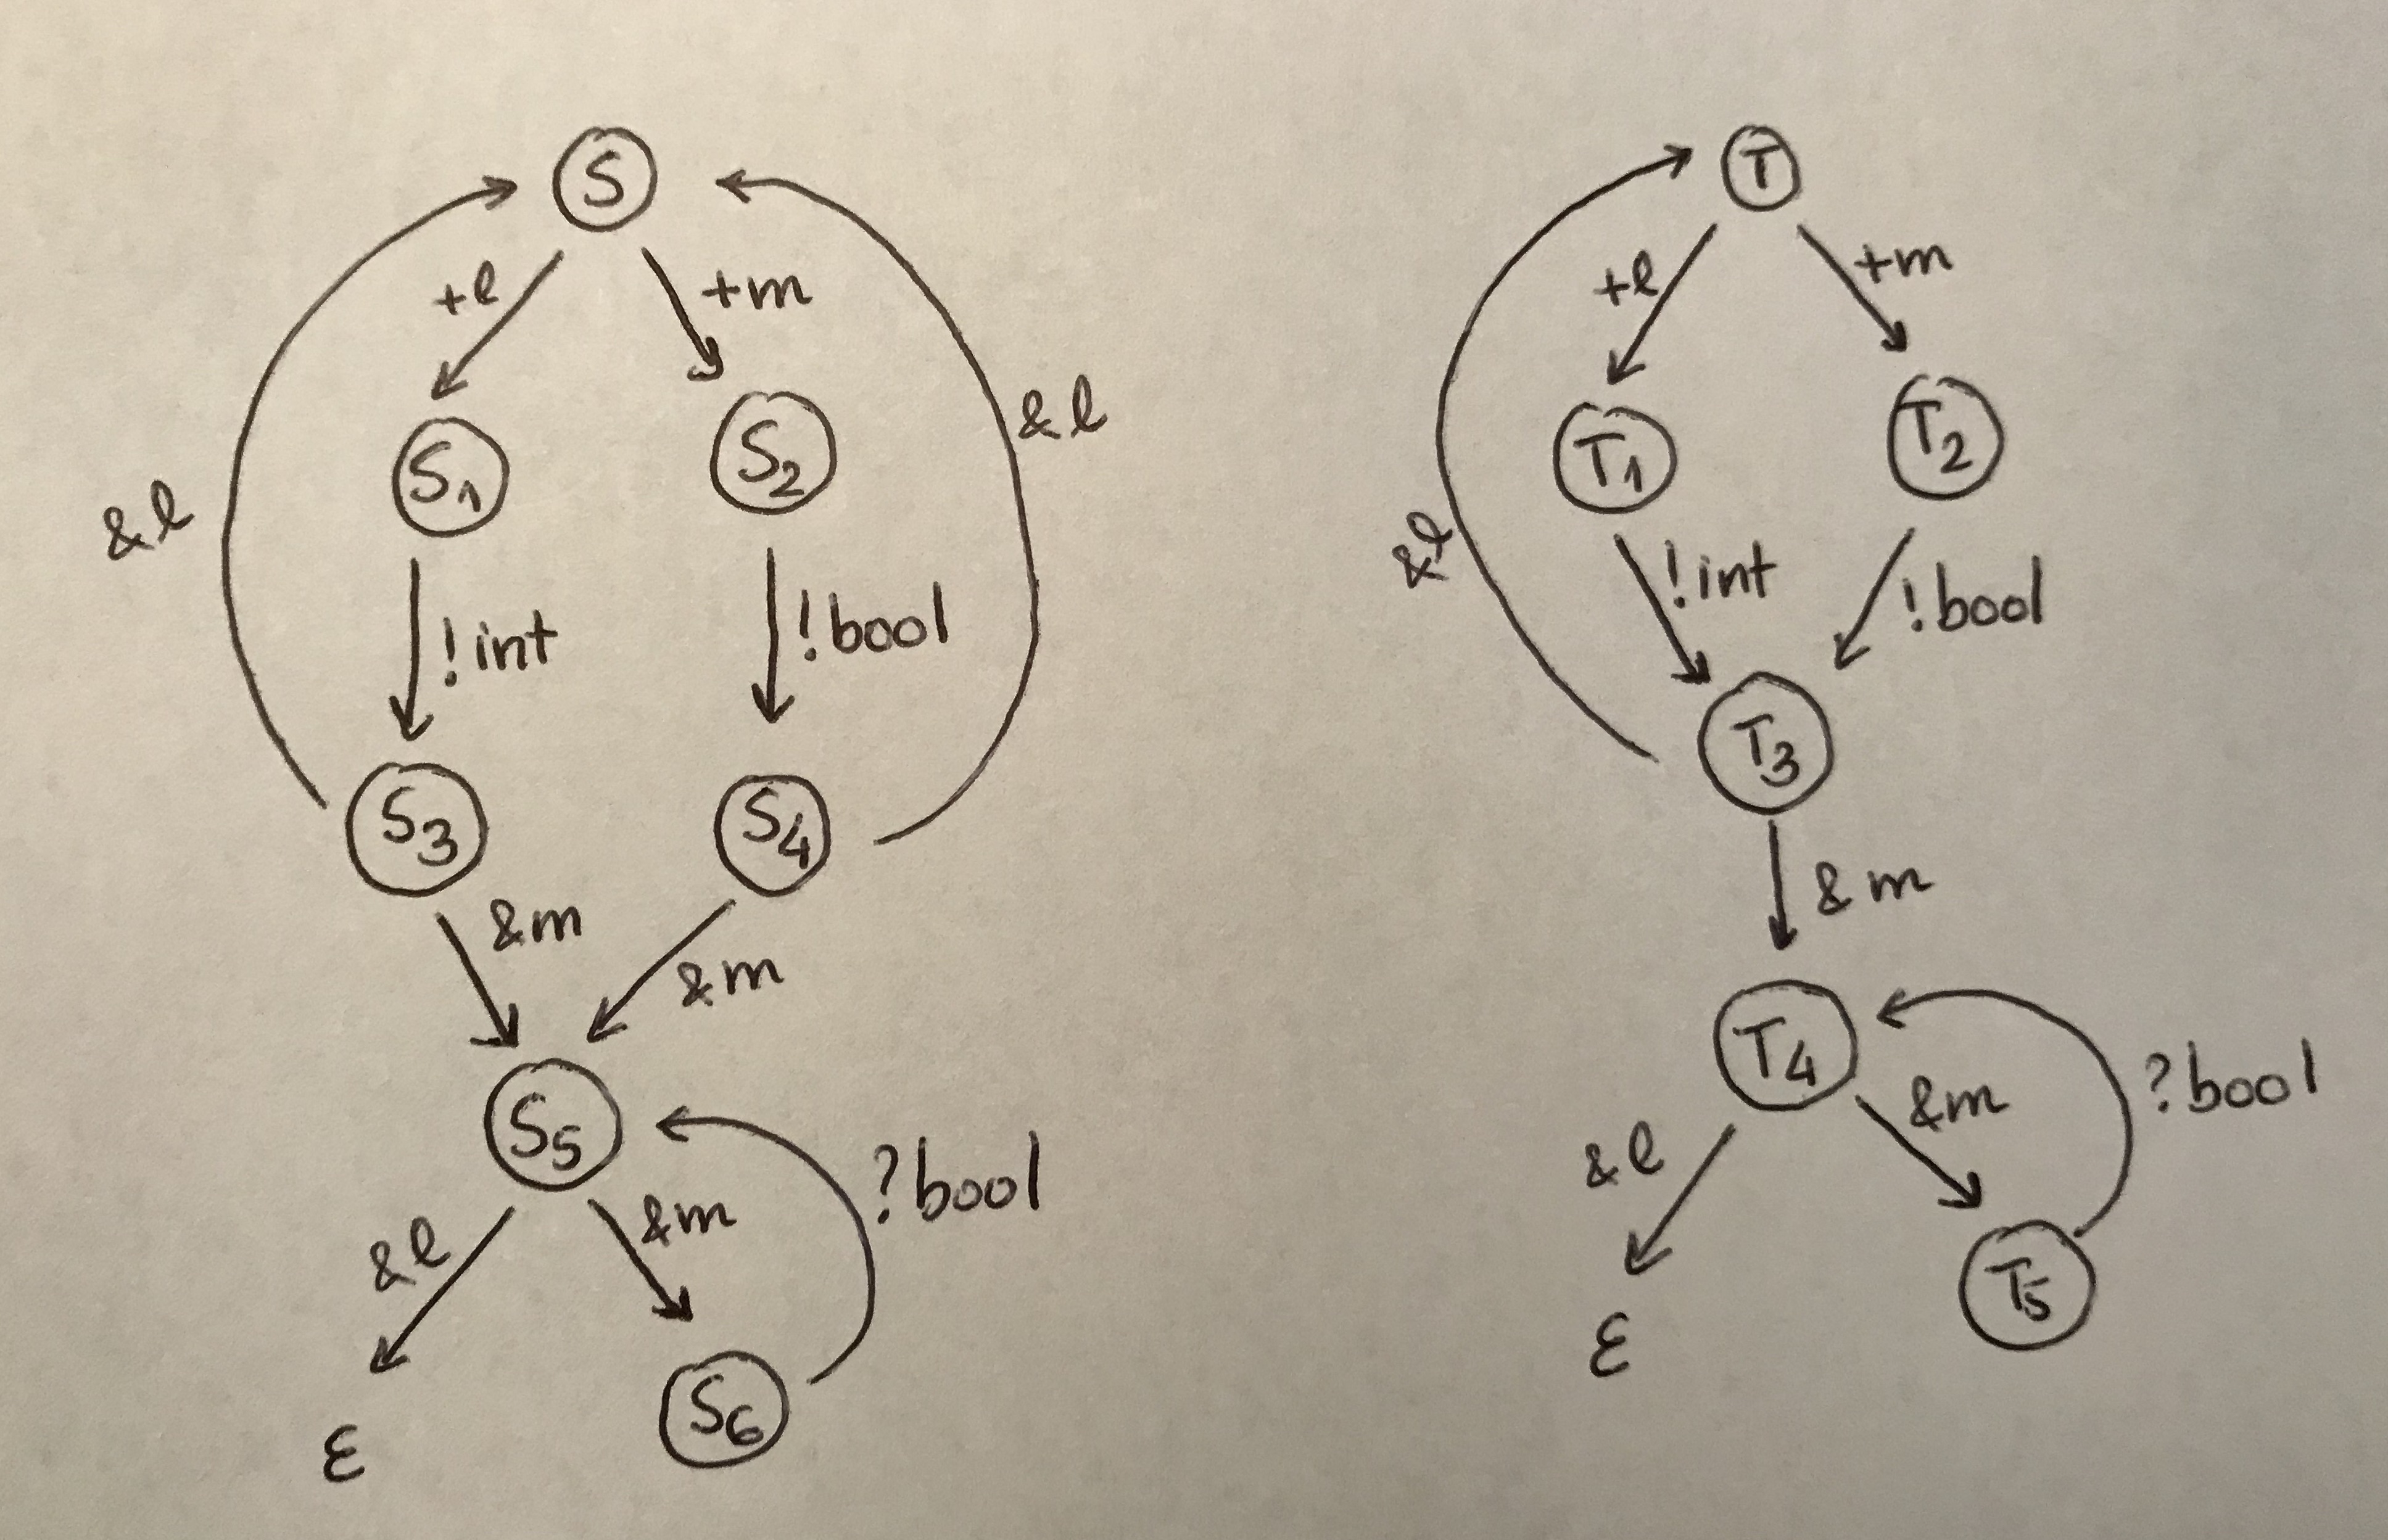
\includegraphics[width=\columnwidth]{PAgraphsST.jpg}
% 		\caption{Process algebra graphs for $S$ and $T$.}
% 			\label{fig:PAgraphsST}
% 	\end{figure}
% 	The algorithm we propose in this work derives the expansion tree for $S\sim T$ as a sequence of nodes. The nodes in this expansion tree can be labeled with a trace of the nodes that lie ahead, based on the syntactical structure of $S$ and $T$. We get the following sequence of labeled nodes in the expansion tree for $S\sim T$:\\\\
% \begin{tikzcd}[cells={nodes={draw=black}}, column sep=large]
%   \enspace (S,T) \enspace \ar[r,"expand"]
% & \enspace  (S_1S_3S_5,T_1T_3), (S_2S_4S_5, T_2T_3) \enspace \ar[r,"expand"]
% & \enspace  (S_3S_5,T_3), (S_4S_5, T_3) \enspace  
% \end{tikzcd} 
% $\xrightarrow{\text{expand}}$\\\\
% \begin{tikzcd}[cells={nodes={draw=black}}, column sep=large]
% & \enspace(SS_5,T),(SS_5,T),(S_5,T_4),(S_5,T_4)  \enspace\ar[r,dashed,"bpa1"]
% &\enspace (S_5,\varepsilon),(S_5,T_4) \enspace 
% \end{tikzcd} 
% $\xrightarrow{\text{expand}}$ \\\\
% \begin{tikzcd}[cells={nodes={draw=black}}, column sep=large]
% &\enspace (S_6S_5,T_5T_4), (\varepsilon,\varepsilon) \enspace \ar[r,dashed,"reflex"] 
% &\enspace (S_6S_5,T_5T_4)\enspace \ar[r,"expand"]
% & \enspace(S_5,T_4)\enspace \ar[r,dashed,"bpa1"]
% &\emptyset\\
% \end{tikzcd}

% 	The process alternates between simplification and expansion operations, denoted by dashed and solid arrows, respectively. Having reached an empty node, we conclude that $S\sim T$.\\\smallskip
	
% 	Now consider the types:
% 	\[ R \triangleq \mu x.\&\{\ell\colon ?\,\boolk;x, m\colon ?\,\intk;x;x \} \text{ and }  U \triangleq \mu x.\&\{\ell\colon ?\,\boolk, m\colon ?\,\intk;x;x\} \enspace .\]
	
% 	$R$ and $U$ are represented as PA graphs as shown in Figure~\ref{fig:PAgraphsRU}.
	
% 	\begin{figure}[h!]
% 	\centering
% 		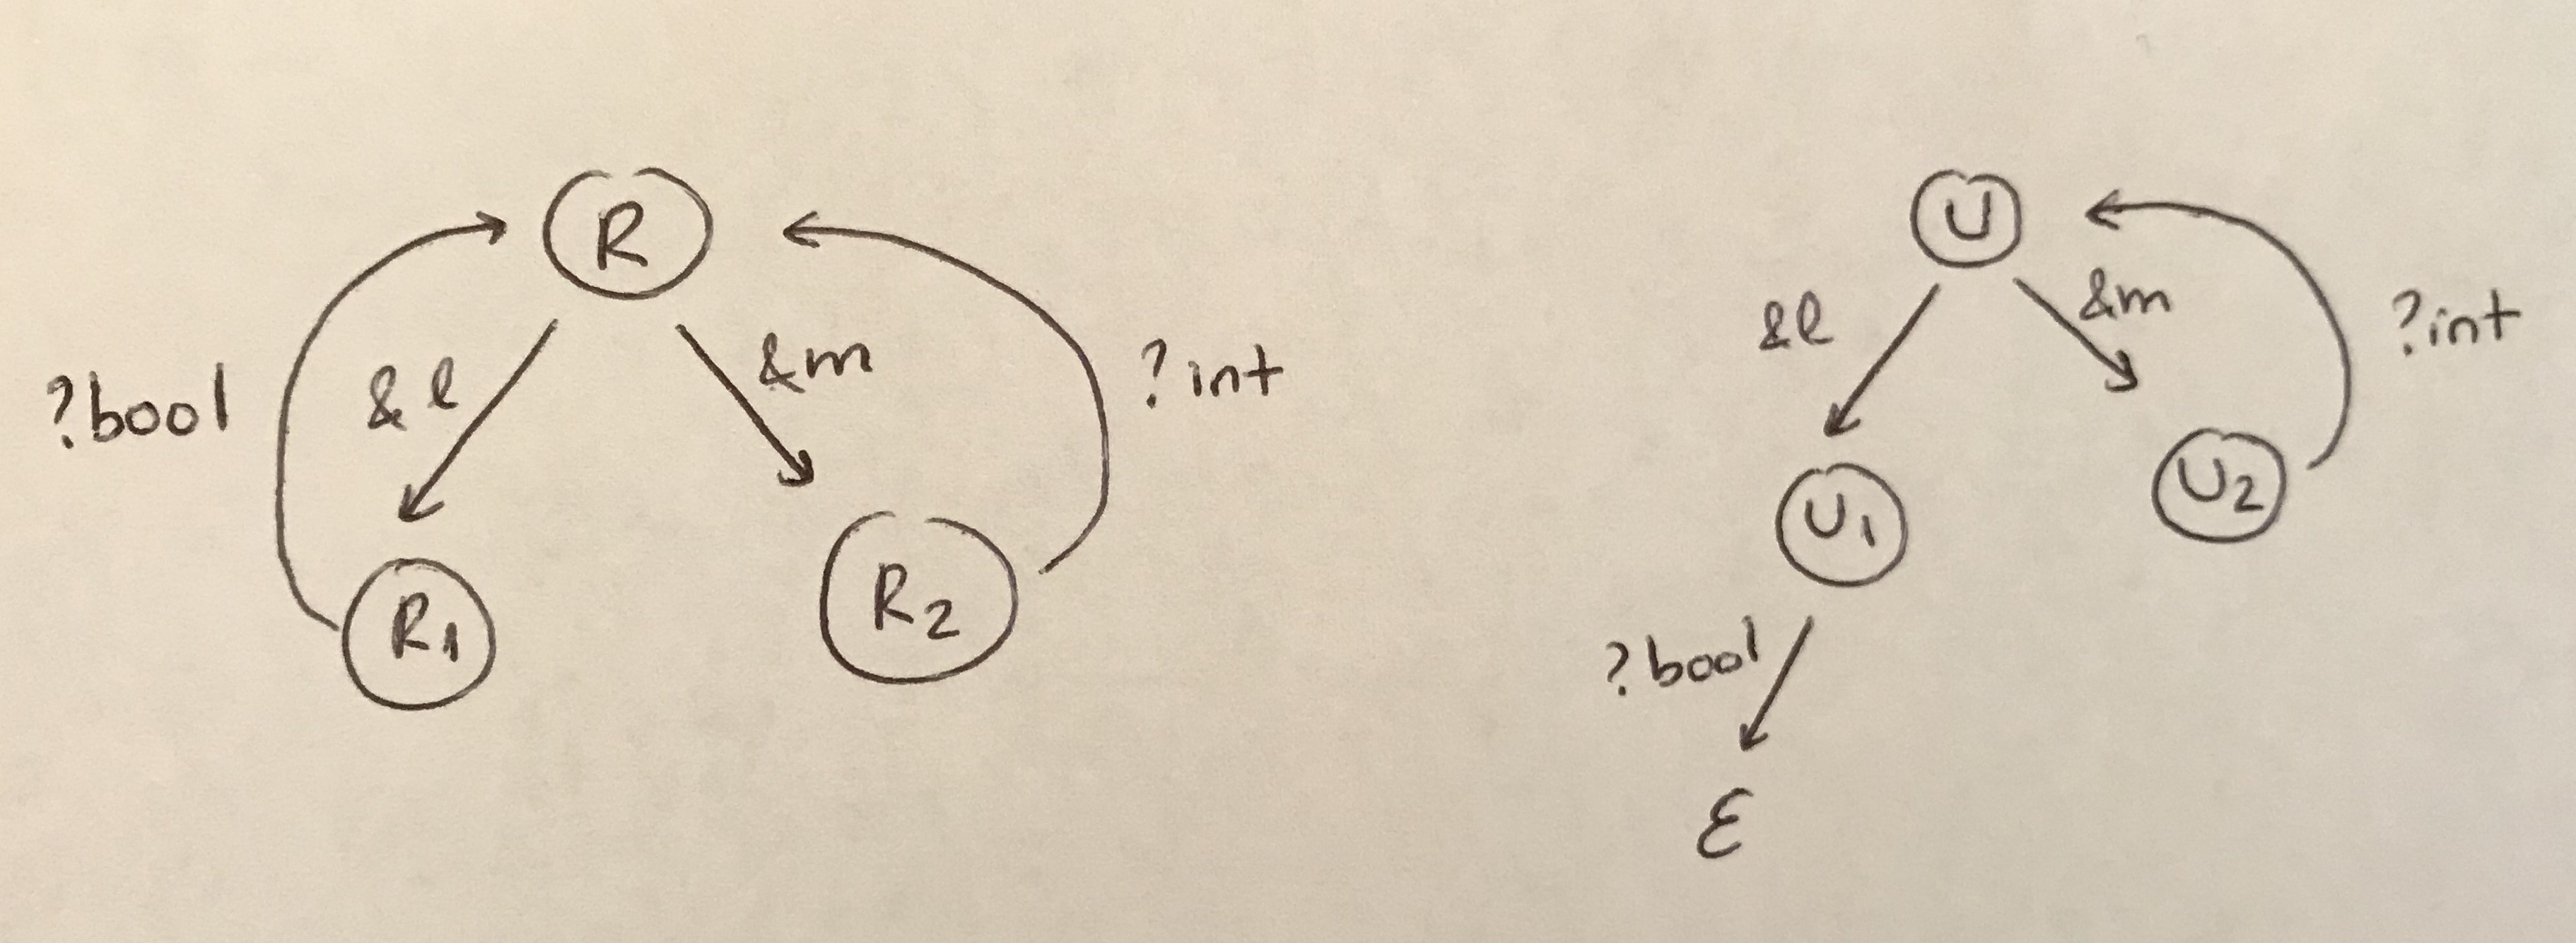
\includegraphics[width=14cm]{PAgraphsRU.jpg}
% 		\caption{Process algebra graphs for $R$ and $U$.}
% 		\label{fig:PAgraphsRU}
% 	\end{figure}
% 	Using the porposed algorithm, we get the following expansion list build upon the syntactical structure of $R$ and $U$ and their representations as PA graphs:\\\\
% \begin{tikzcd}[cells={nodes={draw=black}}, column sep=large]
%   (R,U) \ar[r,"expand"]
% & (R_1 R,U_1), (R_2 R R, U_2 U U) \ar[r,"expand"]
% & (R,\varepsilon), (RR, UU) \ar[r,dashed,"bpa1"] 
% & (R,\varepsilon), (U,\varepsilon) 
% \end{tikzcd} 
% \enspace  $\times$\\\\
% We notice that the last step results from applying BPA1 rule~\cite{janvcar1999techniques} to $(RR,UU)$ knowing that $(R,U)$ is an ancestor node, which leads to the pairs $(R,\varepsilon)$ and $(U,\varepsilon)$. As we then fail to obtain new derived nodes, we decide the type equivalence negatively and conclude that $R\not\sim U$.
% 	\hfill $\triangle$
% \end{example}


%%% Local Variables:
%%% mode: latex
%%% TeX-master: "main"
%%% End:



\end{document}

%%% Local Variables:
%%% mode: latex
%%% TeX-master: t
%%% End:
